\documentclass[letterpaper,11pt]{article}
\pdfoutput=1 % if you are submitting a pdflatex (i.e. if you have  
% images in pdf, png or jpg format)
\usepackage{jheppub}
\usepackage[utf8]{inputenc} 
%\usepackage[T1]{fontenc} % if needed
%\usepackage[latin1]{inputenc}
\usepackage{graphicx}
\usepackage{amsmath}
\usepackage{amsfonts}
\usepackage{slashed}
\usepackage{amssymb}
\usepackage{hyperref}
\hypersetup{colorlinks=true, linkcolor=blue, citecolor=red, urlcolor=cyan, linktoc=page}
%\usepackage{cite}
\usepackage{xfrac}
\usepackage{empheq}
\usepackage{caption, subcaption}

\newcommand{\p}{\partial}
\newcommand{\oi}{\omega_i}
\newcommand{\oj}{\omega_j}
\newcommand{\ok}{\omega_k}
\newcommand{\ol}{\omega_\ell}
\newcommand{\oone}{\overline{\omega}_1}
\newcommand{\otwo}{\overline{\omega}_2}
\newcommand{\thi}{\theta_i}
\newcommand{\thj}{\theta_j}
\newcommand{\thk}{\theta_k}
\newcommand{\thl}{\theta_\ell}
\newcommand{\mc}{\mathcal}
\newcommand{\jm}{\ensuremath{j_{max}}}
\newcommand{\ob}{\overline{\omega}}
\newcommand{\oib}{\overline{\omega}_i}
\newcommand{\ojb}{\overline{\omega}_j}
\newcommand{\okb}{\overline{\omega}_k}
\newcommand{\ib}{\overline{i}}
\newcommand{\jb}{\overline{j}}
\newcommand{\kb}{\overline{k}}
\newcommand{\oal}{\omega_\alpha}
\newcommand{\obet}{\omega_{\beta}}
\newcommand{\ogam}{\omega_\gamma}

%%%%%%%%%%%%%%%%%%%%%%%%%%%%%%%%%%%%%%%%%
%%%%%%%%%%%%%%%%%%%%%%%%%%%%%%%%%%%%%%%%%

\title{Examining Instabilities Due to Driven Scalars in AdS}

\abstract{We extend the study of holographic quantum quenches in AdS to include solutions to driven systems, i.e. those with time-dependent sources on the AdS boundary. This necessitates the activation of non-normalizable modes in the massive bulk scalar field, which then couple to the metric and normalizable scalar modes. Analytic expressions for secular terms that persist after time averaging are determined for scalars in $AdS_{d+1}$ with any mass, and for different driving frequencies. We then numerically evaluate these sources for $d=4$ and discuss what role these play in the perturbative stability of these systems.}

%%%%%%%%%%%%%%%%%%%%%%%%%%%%%%%%%%%%%%%%%
%%%%%%%%%%%%%%%%%%%%%%%%%%%%%%%%%%%%%%%%%

\begin{document}
\maketitle
\flushbottom
\newpage

%%%%%%%%%%%%%%%%%%%%%%%%%%%%%%%%%%%%%%%%%
%%%%%%%%%%%%%%%%%%%%%%%%%%%%%%%%%%%%%%%%%

\section{Introduction}

Examinations of quenches in strongly coupled quantum systems can be approached using the holographic dual of such a process, namely the evolution of weakly coupled gravity. Full accounting of the return to equilibrium -- signalled by the formation of a black hole in the dual theory -- requires advanced numerical methods, and has been the subject of numerous studies. While AdS has been shown to be perturbatively unstable to generic data, an interesting array of stable and meta-stable behaviours that resist gravitational collapse have been demonstrated for initial data close to the fundamental AdS modes, the oscillons. Data that exhibits stability over long times (a scale that is often set by the amplitude of the perturbation) exhibits inverse energy cascades that balance the direct cascade of energy to short length scales. This weakly turbulent energy cascade is captured by the third-order dynamics of a perturbative expansion. To describe the balance of inverse and direct energy flow, a second, ``slow time'' is introduced that governs the evolution of the scalar field and, therefore, the metric functions. This is known as the Two-Time Formulation (TTF), and allows for analytical determination of the evolution of the scalar field in the perturbative regime.

Conventional examinations perturbative stability using TTF have focused on the quenches of some initial energy perturbation. However, the analytic descriptions of holographic pumped solutions -- those with periodic boundary conditions that constantly inject energy into the system -- remains undetermined.  With this in mind, we examine the effect of a time-dependent source on the conformal boundary has on the analytic expressions for the time evolution of the slowly varying integration constants. Quenches in asymptotically AdS spacetime restrict the space of oscillon solutions to those that approach zero near the conformal boundary; however, in a driven solution the energy is pumped into the system through a second class of oscillons: those that approach constant, non-zero values on the boundary. Since these solutions will have non-finite inner products over the space, they are known as non-normalizable solutions. These non-normalizable modes couple to the metric and the normalizable modes to bring energy into the system, where direct and inverse energy cascades proceed over perturbative time scales.

Following the study of resummation and time-averaging procedures for scalar fields in AdS, we isolate secular terms -- those that grow linearly with time and cannot be absorbed by a phase term -- from those that are averaged out. The terms that persist after time averaging are those that obey certain resonance conditions between the frequencies of the non- and normalizable modes. By evaluating the third-order interactions on resonance, we use a renormalization procedure to absorb resonant contributions into the equations for the slowly varying amplitude and phase variables of the scalar field.

This paper is organized as follows: after a brief discussion of how to arrive at the third order source term, we consider the addition of a time-dependent boundary condition for the scalar field. As an exercise, and to provide explicit expressions for our choice of gauge and mass, \S\!~\ref{sec: norm res} examines the resonant contributions in the case of a massive scalar field in AdS$_{d+1}$ with any mass-squared, up to and including the Breitonlohmer-Freedman mass: $m^2_{BF} \leq m^2$. We recover the natural vanishing of two of the three resonances, and then examine the effects of mass-dependence on the non-vanishing channel. Whenever values are calculated, the choice of $d=4$ is implied as to draw the most direct comparison to existing literature. In section~\S\!~\ref{sec: NNmodes}, we extend the boundary conditions to include a variety of periodic boundary sources that couple to non-normalizable modes in the bulk. For each choice of boundary condition, we derive analytic expressions for applicable resonances and evaluate these expressions for different ranges of scalar field masses. Finally, in~\S\!~\ref{sec: discussion} we discuss the implications of non-vanishing resonances on the competing energy cascades and the perturbative stability of such systems. For completeness, we include details of our derivation of the general source term in an appendix, as well as a complete list of possible resonances and their contributions in the case of activating two, equal frequency non-normalizable modes.



%%%%%%%%%%%%%%%%%%%%%%%%%%%%%%%%%%%%%%%%%
%%%%%%%%%%%%%%%%%%%%%%%%%%%%%%%%%%%%%%%%%

\section{Source Terms and Boundary Conditions}

To examine the weak turbulence that leads to instability, we consider a massive scalar field coupled to a spherically symmetric, asymptotically AdS$_{d+1}$ spacetime in global coordinates whose metric is given by
\begin{align}
\label{AdS metric}
ds^2 &= \frac{L^2}{\cos(x)} \left( - A(t,x) e^{-2 \delta(t,x)} \, dt^2 + A^{-1}(t, x) \, dx^2 + \sin^2 (x) \, d\Omega^2_{d-1} \right) \, ,
\end{align}
where $L$ is the AdS curvature (hereafter set to $1$), and the radial coordinate $x \in [0, \pi/2)$. The dynamics of the system come from the Einstein and Klein-Gordon equations:
\begin{align}
G_{\mu \nu} + \Lambda g_{\mu \nu} = 8 \pi \left( \nabla_\mu \phi \nabla_\nu \phi - \frac{1}{2} g_{\mu \nu} \left( \nabla^\rho \phi \nabla_\rho \phi + m^2 \phi^2 \right) \right), \quad \text{and} \quad \nabla^2 \phi - m^2 \phi = 0 \, ,
\end{align}
with $\Lambda$ as cosmological constant for AdS, $\Lambda = -d(d-1)/2$. 

Perturbing around static AdS, we expand the minimally-coupled scalar field in terms of odd powers of epsilon (the even powers do not contribute)
\begin{align}
\phi(t,x) = \epsilon \phi_1 + \epsilon^3 \phi_3 + \ldots
\end{align}
and the metric functions $A$ and $\delta$ in terms of even powers of the expansion parameter,
\begin{align}
A(t, x) = 1 + A_2 \epsilon^2 + \ldots \quad \text{and} \quad \delta(t, x) = \epsilon^2 \delta_2 + \ldots \, .
\end{align}
We choose to work in the boundary gauge, where $\delta(t, \pi/2) = 0$, for reasons that we discuss below.

At linear order, $\phi_1$ satisfies
\begin{align}
\p^2_t \phi_1 + \hat L \phi_1 = 0 \quad \text{where} \quad \hat{L} \equiv \frac{1}{\mu} (\mu' \p_x + \mu \p^2_x)  - \frac{m^2}{\cos^2(x)} \, ,
\end{align}
where $\mu \equiv \tan^{d-1}(x)$. Writing the scalar field as the product of time- and position-dependent parts,
\begin{align}
\phi_1 (t, x) = \sum_j c_j (t) e_j (x) \, ,
\end{align}
we find that the basis functions $e_j (x)$ are the solutions to the eigenvalue equation
\begin{align}
\label{eigen eqn}
\hat L e_j(x) = \omega^2_j e_j(x) .
\end{align}
The general solution to this eigenvalue equation involves two types of functions: those that are normalizable and therefore vanish as $x \to \pi / 2$, and those that are non-normalizable and approach a finite value on the boundary. In many previous works, the dynamics of scalar fields have been studied using exclusively normalizable functions (as is the focus of \S\!~\ref{sec: norm res}); however, we now wish to consider so-called ``pumped'' systems, where a time-dependent source term exists on the boundary that sends energy into AdS. This energy is carried into the bulk spacetime via non-normalizable solutions to \eqref{eigen eqn}, and coupling between the scalar field and metric functions drives the system out of equilibrium. 

In general, a combination of normalizable and non-normalizable eigenmodes make up the scalar field:
\begin{align}
\phi_1(t,x) = \sum_j c_j(t) e_j(x) + \sum_\alpha \bar A_\alpha (t) E_\alpha(x) \, ,
\end{align}
with the $\bar A_\alpha$ set by the choice of boundary conditions. The normalizable modes have eigenfunctions given by
\begin{align}
e_j(x) &= k_j \left( \cos(x) \right)^{\Delta^+} P_{j}^{(d/2 - 1, \, \Delta^+ - d/2)} \left( \cos (2x) \right) \\
k_j &= 2 \sqrt{\frac{(j + \Delta^+ /2) \Gamma(j+1) \Gamma(j+\Delta^+)}{\Gamma(j+d/2) \Gamma(j + \Delta^+ - d/2 + 1)}} \, ,
\end{align} 
with fully resonance eigenvalues $\omega_j = 2j + \Delta^+$, $j \in \mathbb{Z}^*$, and $\Delta^+$ as the positive root of $\Delta ( \Delta - d ) = m^2$. On the other hand, non-normalizable eigenfunctions with arbitrary frequency $\omega_\alpha$, have basis functions
\begin{align}
\label{general basis}
E_\alpha (x) =  \left( \cos(x) \right)^{\Delta_+} {_2F_1} \left(\frac{\Delta_+ + \omega_\alpha}{2}, \frac{\Delta_+ - \omega_\alpha}{2}, d/2 ; \sin^2 (x) \right) \, .
\end{align}

\begin{center}
{\bf DISCUSS RESONANT CONTRIBUTIONS \& THE TIME AVERAGING PROCEDURE}
\end{center}

Without specifying whether an eigenmode is non-/normalizable, we can determine the effect of the weakly turbulent transfer of energy at $\mc O(\epsilon^3)$, with
\begin{align}
\ddot \phi_3 + \hat L \phi_3 = S = 2 (A_2 - \delta_2) \ddot \phi_1 + (\dot A_2 - \dot \delta_2) \dot\phi_1 + (A_2' -\delta_2' )\phi_1' + m^2 A_2 \phi_1 \sec^2 x \, .
\end{align}
Following the steps outlined in Appendix~\ref{app: source term derivation}, and employing the solution ${c_i(t) = a_i \cos (\oi t + b_i) = a_i \cos\theta_i}$, the source term can be written as
\begin{align}
\label{general source}
S_\ell &=\frac{1}{4} \sum_{\substack{i,j,k \\ k \neq \ell}}^\infty \frac{a_i a_j a_k \ok}{\ol^2 - \ok^2} \Big[ Z^-_{ijk\ell} (\oi + \oj - 2\ok) \cos (\thi + \thj - \thk) - Z^-_{ijk\ell} (\oi + \oj + 2\ok) \cos (\thi + \thj + \thk) - \nonumber \\
%
&\qquad + Z^+_{ijk\ell} (\oi - \oj + 2\ok)  \cos(\thi - \thj + \thk) - Z^+_{ijk\ell} (\oi - \oj - 2\ok) \cos (\thi - \thj - \thk) \Big] \nonumber \\
%
& + \frac{1}{2}\sum_{\substack{i,j,k \\ i \neq j}}^\infty a_i a_j a_k \oj \left( H_{ijk\ell} + m^2 V_{jki\ell} - 2\ok^2 X_{ijk\ell} \right) \Big[ \frac{1}{\oi - \oj} \left( \cos (\thi - \thj - \thk)  + \cos(\thi - \thj + \thk) \right) \nonumber \\
%
& \qquad - \frac{1}{\oi + \oj} \left( \cos (\thi + \thj - \thk)  + \cos ( \thi + \thj + \thk) \right) \Big] \nonumber \\
%
& - \frac{1}{4} \sum_{i,j,k}^\infty a_i a_j a_k \Big[ \left( 2\oj \ok X_{ijk\ell} + m^2 V_{ijk\ell} \right)\cos(\thi + \thj - \thk) -  \left( 2\oj\ok X_{ijk\ell} - m^2 V_{ijk\ell} \right) \cos(\thi - \thj - \thk) \nonumber \\
%
& \qquad + \left(2\oj \ok X_{ijk\ell} + m^2 V_{ijk\ell} \right) \cos (\thi - \thj + \thk) - \left( 2\oj\ok X_{ijk\ell} - m^2 V_{ijk\ell} \right) \cos(\thi + \thj + \thk) \Big] \nonumber \\
%
& + \frac{1}{4} \sum_{i,j}^\infty a_i a_j a_\ell \ol \Big[ \tilde Z^-_{ij\ell} (\oi + \oj - 2\ol) \cos (\thi + \thj - \thl) - \tilde Z^-_{ij\ell} (\oi + \oj + 2\ol) \cos(\thi + \thj +  \thl) \nonumber \\
%
& \qquad + \tilde Z^+_{ij\ell} (\oi - \oj + 2\ol) \cos(\thi - \thj + \thl)  - \tilde Z^+_{ij\ell} (\oi - \oj - 2\ol) \cos( \thi - \thj - \thl)  \Big] \nonumber \\
%
& - \frac{1}{4} \sum_{i,j}^\infty a_i^2 a_j \left( H_{iij\ell} + m^2 V_{jii\ell} - 2\oj^2 X_{iij\ell} \right) \big[ \cos (2\thi - \thj) + \cos (2\thi + \thj) \big] \nonumber \\
%
& - \frac{1}{2} \sum_{i,j}^\infty a_i^2 a_j \left( H_{iij\ell} + m^2 V_{jii\ell} - 2\oj^2 X_{iij\ell} + 4\oi^2 \oj^2 P_{j\ell i} + 2\oi^2 (M_{j\ell i} + m^2 Q_{j\ell i}) \right) \cos \thj . \hspace{-0.2in}
\end{align} 

As an exercise, we first derive the resonant contributions when the boundary source is zero, and therefore only normalizable modes are present. These results agree numerically with previous work on normalizable modes for massless scalars in the interior time gauge $\delta(t, 0) = 0$. The definitions of the integral functions $Z$, $H$, $X$, etc. differ slightly from other works -- in part because of the gauge choice, and in part because of a desire to separate mass-dependent terms -- and so are given explicitly in Appendix~\ref{app: source term derivation}.

%%%%%%%%%%%%%%%%%%%%%%%%%%%%%%%%%%%%%%%%%
%%%%%%%%%%%%%%%%%%%%%%%%%%%%%%%%%%%%%%%%%

\section{Resonances From Normalizable Solutions}
\label{sec: norm res}
Consider the case where each of the basis functions are given by normalizable solutions. After time-averaging, the  resonant contributions occur for the following combination of normalizable frequencies: 
\begin{align}
\label{gen res}
\oi \pm \oj \pm \ok = \pm \ol \,
\end{align}
which can be separated into the three distinct cases
\begin{align}
\oi + \oj + \ok &= \ol \qquad (+++) \\
\oi - \oj - \ok &= \ol \qquad (+--) \\
\oi + \oj - \ok &= \ol \qquad (++-) \, .
\end{align}
We will see that the first two resonances, $(+++)$ and $(+--)$, will non-trivially vanish whenever their respective resonance conditions are satisfied. This is in agreement with the results shown for the massless scalar in the interior time gauge (as they must be, since the choice of time gauge should not change the existence of resonant channels). Here we include the expressions for the naturally vanishing resonances, choosing to explicitly express the mass dependence.

%%%%%%%%%%%%%%%%%%%%%%%%%%%%%%%%%%%%%%%%%

\subsection{Naturally Vanishing Resonances: $(+++)$ and $(+--)$}

Resonant contributions that come from the condition $\oi + \oj + \ok = \ol$ are of the form
\begin{align}
S_\ell = \underbrace{\sum_{i=0}^\infty \sum_{j=0}^\infty \sum_{k=0}^\infty}_{\oi + \oj + \ok = \, \ol} \Omega_{ijk\ell} \, a_i a_j a_k \cos \left( \thi + \thj + \thk \right) + \ldots \, ,
\end{align}
where dots denote other resonances, both vanishing and non-vanishing. $\Omega_{ijk\ell}$ is then given by
\begin{align}
\label{omega}
\Omega_{ijk\ell} &= -\frac{1}{12}H_{ijk\ell} \frac{\oj (\oi + \ok +2\oj)}{(\oi + \oj)(\oj + \ok)} - \frac{1}{12} H_{ikj\ell} \frac{\ok (\oi + \oj + 2\ok)}{(\oi + \ok)(\oj + \ok)}- \frac{1}{12} H_{jik\ell} \frac{\oi (\oj + \ok +2\oi)}{(\oi + \oj)(\oi + \ok)} \nonumber \\
%
& \quad - \frac{m^2}{12} V_{ijk\ell} \left( 1 + \frac{\oj}{\oj + \ok} + \frac{\oi}{\oi + \ok} \right) - \frac{m^2}{12} V_{jki\ell} \left( 1 + \frac{\oj}{\oi + \oj} + \frac{\ok}{\oi + \ok} \right) \nonumber \\
%
& \quad - \frac{m^2}{12} V_{kij\ell} \left( 1 + \frac{\oi}{\oi + \oj} + \frac{\ok}{\oj + \ok} \right)  + \frac{1}{6} \oj \ok X_{ijk\ell} \left( 1 + \frac{\oj}{\oi + \ok} + \frac{\ok}{\oi + \oj} \right) \nonumber \\
%
& \quad + \frac{1}{6} \oi \ok X_{jki\ell} \left( 1 + \frac{\oi}{\oj + \ok} + \frac{\ok}{\oi + \oj} \right) + \frac{1}{6} \oi \oj X_{kij\ell} \left( 1 + \frac{\oi}{\oj + \ok} + \frac{\oj}{\oi + \ok} \right) \nonumber \\
%
& \quad - \frac{1}{12} Z^-_{ijk\ell} \left( \frac{\ok}{\oi + \oj} \right) - \frac{1}{12} Z^-_{ikj\ell} \left( \frac{\oj}{\oi + \ok} \right) - \frac{1}{12} Z^-_{jki\ell}  \left( \frac{\oi}{\oj + \ok} \right) \, .
\end{align}

The second naturally vanishing resonance comes from the condition $\oi - \oj - \ok = \ol$, and is of the form
\begin{align}
S_\ell = \sum_{j=0}^\infty \sum_{k=0}^\infty \Gamma_{(j + k + \ell + \Delta^+) jk\ell} \, a_j a_k a_{(j+k+\ell + \Delta^+)} \cos \left( \theta_{(j+k+\ell + \Delta^+)} - \thj - \thk \right) + \ldots \, ,
\end{align}
where
\begin{align}
\label{gamma}
\Gamma_{ijk\ell} &= \frac{1}{4} H_{ijk\ell} \frac{\oj (\ok - \oi + 2\oj)}{(\oi - \oj)(\oj + \ok)} + \frac{1}{4} H_{jki\ell} \frac{\ok (\oj - \oi + 2\ok)}{(\oi - \ok)(\oj + \ok)} + \frac{1}{4} H_{kij\ell} \frac{\oi (\oj + \ok - 2\oi)}{(\oi - \oj)(\oi - \ok)} \nonumber \\
% 
& \quad -\frac{1}{2} \oj \ok X_{ijk\ell} \left( \frac{\ok}{\oi - \oj} + \frac{\oj}{\oi - \ok} - 1\right) + \frac{1}{2} \oi \ok X_{jki\ell} \left( \frac{\ok}{\oi - \oj} + \frac{\oi}{\oj + \ok} - 1 \right) \nonumber \\
%
& \quad + \frac{1}{2} \oi \oj X_{kij\ell} \left( \frac{\oj}{\oi - \ok} + \frac{\oi}{\oj + \ok} -1 \right) + \frac{m^2}{4} V_{jki\ell} \left( \frac{\oj}{\oi - \oj} + \frac{\ok}{\oi - \ok} -1\right) \nonumber \\
%
& \quad - \frac{m^2}{4} V_{kij\ell} \left( \frac{\oi}{\oi - \oj} + \frac{\ok}{\oj + \ok} + 1\right) - \frac{m^2}{4} V_{ijk\ell} \left( \frac{\oi}{\oi - \ok} + \frac{\oj}{\oj + \ok} + 1 \right) \nonumber \\
%
& \quad + \frac{1}{4} Z^-_{kji\ell} \left( \frac{\oi}{\oj + \ok}\right) - \frac{1}{4} Z^+_{ijk\ell} \left( \frac{\ok}{\oi - \oj} \right) - \frac{1}{4} Z^+_{jki\ell} \left( \frac{\oj}{\oi - \ok}\right) \, .
\end{align}

Building on the work done with massless scalars, we are able to demonstrate that \eqref{omega} and \eqref{gamma} continue to vanish for massive scalars in the boundary gauge; thus, the weak turbulence is determined only from the remaining resonance channel. When non-normalizable modes are introduced, we will see that naturally vanishing resonances are not present.

%%%%%%%%%%%%%%%%%%%%%%%%%%%%%%%%%%%%%%%%%

\subsection{$(++-)$}
\label{subs: ttf resonances}

The first non-vanishing contributions arise when $\oi + \oj = \ok + \ol$. This contribution can be split into three coefficients that are evaluated for certain subsets of the allowed values for the indices, namely
\begin{align}
S_\ell &= T_\ell a^3_\ell \cos (\thl + \thl - \thl) + \sum_{i \neq \ell}^\infty R_{i \ell} \, a^2_i a_\ell \cos(\thi + \thl - \thi) \nonumber \\
& \qquad + \sum_{i \neq \ell}^\infty \sum_{j \neq \ell}^\infty S_{i j (i + j - \ell) \ell} \, a_i a_j a_{(i + j - \ell)} \cos(\thi + \thj - \theta_{i + j -\ell} ) + \ldots
\end{align}
where each of the coefficients is given by
\begin{align}
\label{S_ppm}
S_{ijk\ell} &= - \frac{1}{4} H_{kij\ell} \frac{\oi (\oj - \ok + 2\oi)}{(\oi - \ok)(\oi + \oj)} -\frac{1}{4} H_{ijk\ell} \frac{\oj (\oi - \ok + 2\oj)}{(\oj - \ok)(\oi + \oj)} - \frac{1}{4} H_{jki\ell} \frac{\ok ( \oi + \oj - 2\ok)}{(\oi - \ok)(\oj - \ok)} \nonumber \\
%
& \quad - \frac{1}{2} \oj \ok X_{ijk\ell} \left( \frac{\oj}{\oi - \ok} - \frac{\ok}{\oi + \oj} + 1 \right) - \frac{1}{2} \oi \ok X_{jki\ell} \left( \frac{\oi}{\oj - \ok} - \frac{\ok}{\oi + \oj} + 1 \right) \nonumber \\
%
& \quad + \frac{1}{2} \oi \oj X_{kij\ell} \left( \frac{\oi}{\oj - \ok} + \frac{\oj}{\oi - \ok} + 1 \right) - \frac{m^2}{4} V_{ijk\ell} \left( \frac{\oi}{\oi - \ok} + \frac{\oj}{\oj - \ok} + 1\right) \nonumber \\
%
& \quad + \frac{m^2}{4} V_{jki\ell} \left( \frac{\ok}{\oi - \ok} - \frac{\oj}{\oi + \oj} - 1 \right) + \frac{m^2}{4} V_{kij\ell} \left( \frac{\ok}{\oj - \ok} - \frac{\oi}{\oi + \oj} - 1 \right) \nonumber \\
%
& \quad + \frac{1}{4}  Z^-_{ijk\ell} \left( \frac{\ok}{\oi + \oj}\right)  + \frac{1}{4}  Z^+_{ikj\ell} \left( \frac{\oj}{\oi - \ok}\right) + \frac{1}{4} Z^+_{jki\ell} \left( \frac{\oi}{\oj - \ok} \right) \, ,
\end{align}
\begin{align}
\label{R_ppm}
R_{i\ell} &= \left(\frac{\oi^2}{\ol^2 - \oi^2} \right) \big( Y_{i\ell \ell i} - Y_{i\ell i \ell} + \ol^2 ( X_{i\ell i \ell} - X_{\ell i \ell i}) \big) + \left(\frac{\oi^2}{\ol^2 - \oi^2}\right) \big( H_{\ell i i\ell} + m^2 V_{ii\ell \ell} - 2\oi^2 X_{\ell i i \ell} \big) \nonumber \\
%
& - \left(\frac{\ol^2}{\ol^2 - \oi^2} \right) \big( H_{i\ell i \ell} + m^2 V_{\ell i i \ell} - 2\oi^2 X_{i\ell i\ell} \big) - \frac{m^2}{4}(V_{i\ell i \ell} + V_{ii\ell \ell} ) + \oi^2 \ol^2 (P_{ii\ell} - 2P_{\ell \ell i}) \nonumber \\
%
& - \oi\ol X_{i\ell i \ell} - \frac{3m^2}{2} V_{\ell ii \ell} - \frac{1}{2} H_{ii\ell \ell} + \ol^2 B_{ii\ell} - \oi^2 M_{\ell \ell i} - m^2 \oi^2 Q_{\ell \ell i} \, ,
\end{align}
and
\begin{align}
\label{T_ppm}
T_{\ell} &= \frac{1}{2} \ol^2 \left( X_{\ell \ell \ell \ell} + 4 B_{\ell \ell \ell} -2 M_{\ell \ell \ell} - 2m^2 Q_{\ell \ell \ell} \right) -\frac{3}{4} \left( H_{\ell \ell \ell \ell} + 3m^2 V_{\ell \ell \ell \ell} \right) \, .
\end{align}

To examine the effects of non-zero masses on $R$, $S$, and $T$ -- and therefore the differential equations that determine the evolution of the time-dependent coefficients $a_i(t)$ and $b_i(t)$ -- we evaluate \eqref{S_ppm}-\eqref{T_ppm} for tachyonic, massless, and massive scalars in figure~\ref{fig: Nmodes}.

\begin{figure}
\centering
	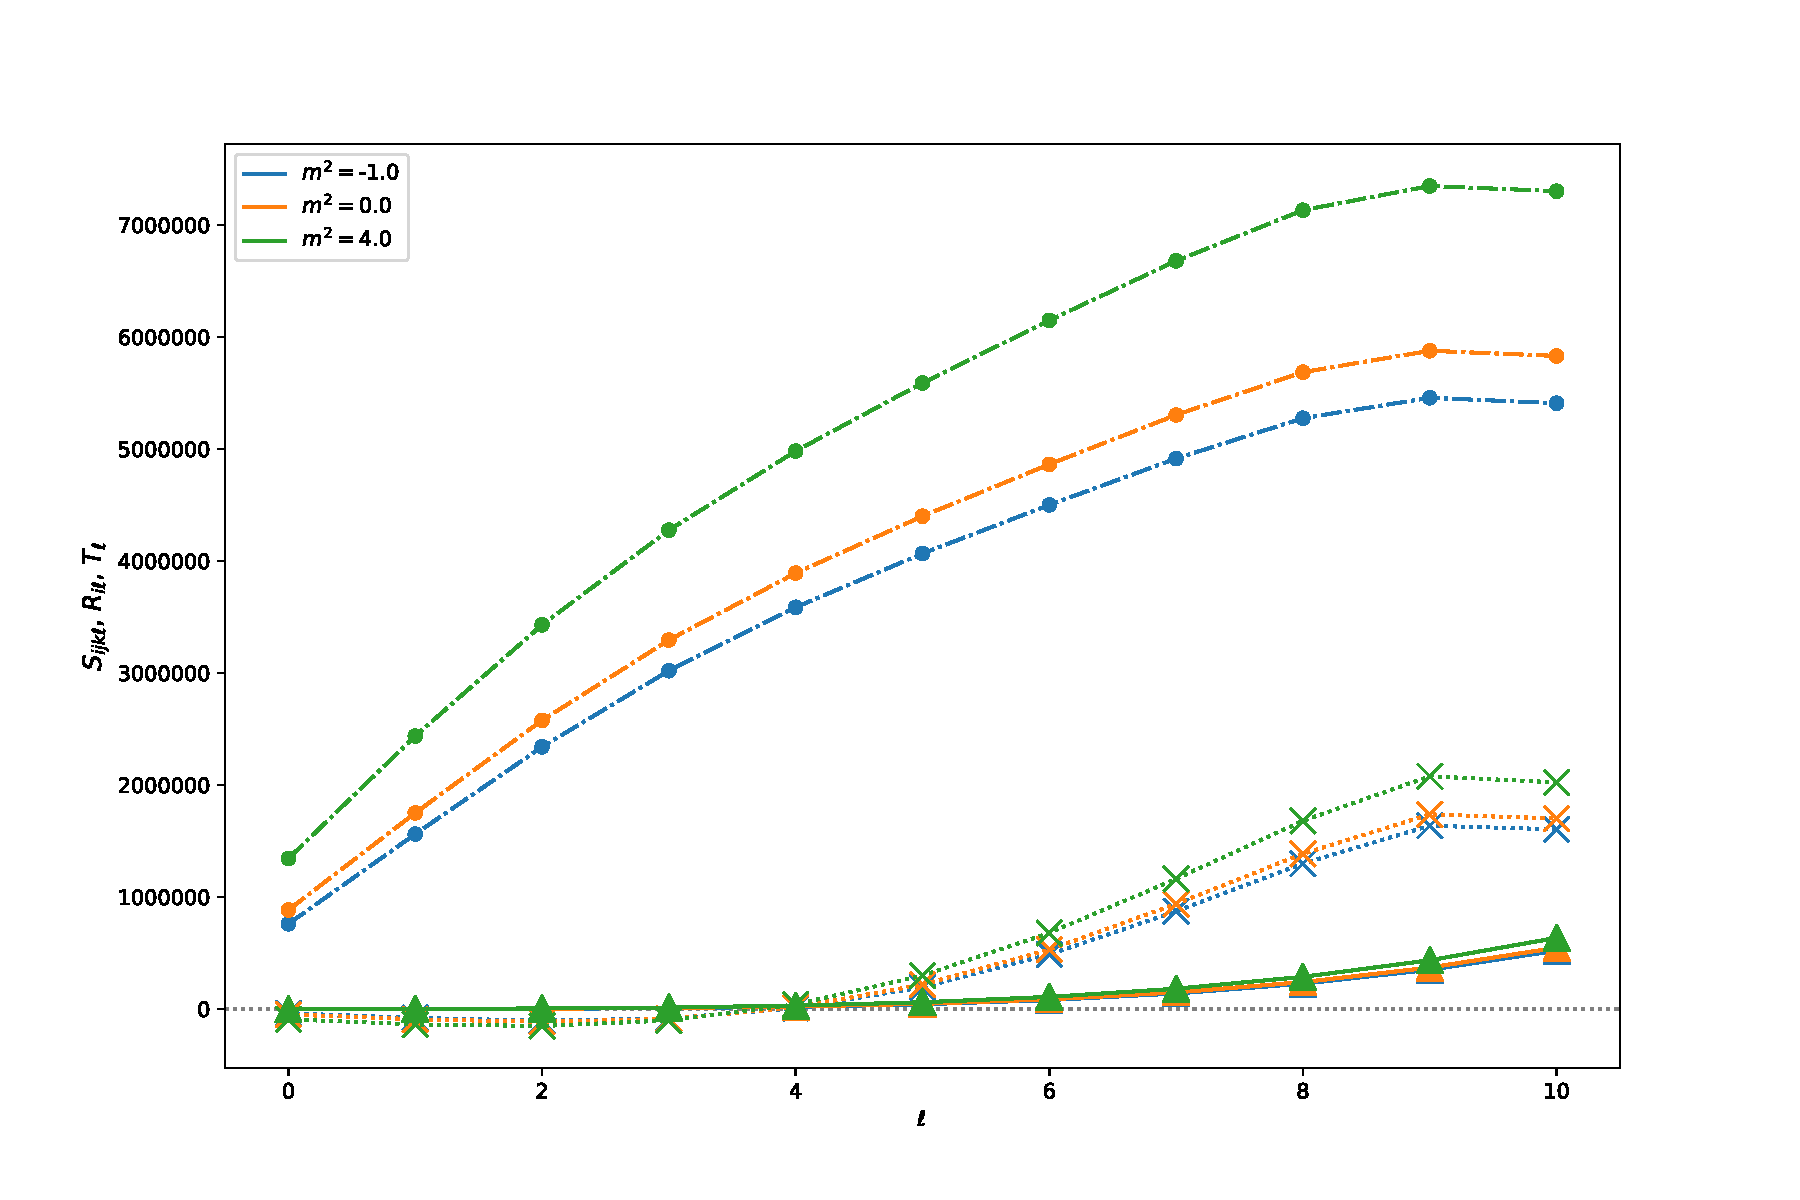
\includegraphics[width=\textwidth]{./figures/Nmodesplot}
	\caption{Evaluating \eqref{S_ppm}-\eqref{T_ppm} for three different values of $m^2$ for $\ell \leq 10$. $S_{ij(i+j-\ell)\ell}$ is denoted by filled circles connected by dash-dotted lines; $R_{i\ell}$ is denoted by filled triangles connected by solid lines; $T_{\ell}$ is denoted by large Xs connected by dotted lines.}
	\label{fig: Nmodes}
\end{figure}


%%%%%%%%%%%%%%%%%%%%%%%%%%%%%%%%%%%%%%%%%
%%%%%%%%%%%%%%%%%%%%%%%%%%%%%%%%%%%%%%%%%

\section{Resonances From Non-normalizable Modes}
\label{sec: NNmodes}

\begin{center}
{\bf Discuss falloff of A2 and delta2 with three NN modes, but don't calculate anything new. Mention overlap of NN and normalizable cases when omega(i) $\pm$ omega(j) = NN frequency. Then focus on two NN modes.}
\end{center}

We now consider the case when at least one of the $e_i(x), e_j(x), e_k(x)$ is a non-normalizable mode. Since the boundary condition has been set to be a single non-normalizable mode, any non-normalizable modes in the source term must exactly cancel; therefore, at least two of the modes must be non-normalizable. This assumption breaks some of the symmetries that contributed to the previous expressions for resonance channels, and so the resonance conditions must be re-examined starting from the source expression \eqref{general source}.

An important consideration is also the effect of non-normalizable modes on the perturbative expansion that leads to the source equations. Since non-normalizable solutions do not have well-defined norms, we do not know \emph{a priori} that the inner products described in Appendix~\ref{app: source term derivation} are still finite. To investigate this, consider the second-order metric function
\begin{align}
A_2 &= - \nu \int^x_0 dy \, \mu \left( (\dot \phi_1)^2 + (\phi'_1)^2 + m^2 \phi_1^2 \sec^2 x \right) \, ,
\end{align}
in the limit of $x \to \pi/2$ when the scalar field is given by a generic superposition of normalizable and non-normalizable eigenfunctions:
\begin{align}
\phi_1 (t, x) &= \sum_\alpha e_\alpha \cos (\omega_\alpha t ) + \sum_i a_i e_i \cos (\omega_i t + b_i) \, .
\end{align}
Focusing on the position-dependence only, we find that
\begin{align}
\lim_{\tilde x \to 0} A_2 (\tilde x = \pi /2 - x) = \tilde{x}^{-\xi} \left( \frac{2 \tilde{x}^{2+d}}{2 - \xi} - \frac{\tilde{x}^d (1 + \left(\Delta^{-}\right)^2)}{\xi} \right)
\end{align}
where we have defined $\xi = \sqrt{d^2 + 4m^2}$. In the massless case, $\xi = d$ and all powers of $\tilde{x}$ are non-negative and thus the limit is finite; for tachyonic masses, $0 \leq \xi < d$ and the limit is again finite. However, for massive scalars, at least one of the terms above diverges as $\xi \to 0$. This case would require the addition of counter-terms in the bulk action to cancel such divergences -- we will not consider this case presently. Thus, we will restrict our discussion to $m^2 \leq 0$ to avoid these issues. A similar check on the near-boundary behaviour of $\delta_2$ shows that, in the massless case, the gauge condition $\delta_2 (t, x=\pi/2)$ remains unchanged by the addition of non-normalizable modes.

\subsection{Two Non-normalizable Modes with Equal Frequencies}
\label{ssec: equalNN}

As a first case, let us assume that the two non-normalizable modes have equal, constant, and arbitrary frequencies, $\ob$. Applying the time-averaging procedure to the source $S_\ell$ once again eliminates all contributions except those that satisfy \eqref{gen res}. Since the basis onto which we are projecting is normalizable, we know that $\omega_\ell$ is given by $\omega_\ell = 2\ell + \Delta^{+}$. We are now free to choose any one of $\{\omega_i, \omega_j, \ok\}$ to be normalizable and consider when the resonance condition is satisfied. In particular, we find that the following combinations are resonant:
\begin{align}
\label{gen nn res 1}
\oi - \oj + \ok - \ol &= 0 \qquad \Rightarrow \qquad \text{either $\oi$ or $\ok$ is normalizable} \\
\oi + \oj - \ok - \ol &= 0 \qquad \Rightarrow \qquad \text{either $\oi$ or $\oj$ is normalizable} \\
\oi - \oj - \ok + \ol &= 0 \qquad \Rightarrow \qquad \text{either $\oj$ or $\ok$ is normalizable.}
\label{gen nn res 2}
\end{align}
When any of these resonance conditions is met, the remaining normalizable mode will have a frequency equal to $\ol$, collapsing all sums over frequencies so that
\begin{align}
\label{2genNN}
S_\ell = \overline{T}_{\ell} \, a_\ell \bar A_{\ob}^2 \cos (\thl) \, ,
\end{align}
where the non-normalizable modes have constant amplitudes $\bar A_{\ob}$. Collecting the appropriate terms in \eqref{general source}, and evaluating the each possible resonance (being careful not to violate restrictions placed on the sums), we find that
\begin{align}
\label{S:2NN}
\overline{T}_{\ell} &=  \bigg[ \, \frac{1}{2} Z^-_{\ell\ob\ob\ell} \left( \frac{\ob}{\ol + \ob} \right) + \frac{1}{2} Z^+_{\ell\ob\ob\ell} \left( \frac{\ob}{\ol - \ob} \right)  + H_{\ell \ob \ob \ell} \left( \frac{\ob^2}{\ol^2 - \ob^2} \right)  - H_{\ob\ell\ob\ell} \left(\frac{\ol^2}{\ol^2 - \ob^2} \right) \nonumber \\
%
& - m^2 V_{\ell \ob\ob\ell}  \left(\frac{\ol^2}{\ol^2 - \ob^2} \right) + m^2 V_{\ob\ob\ell\ell} \left( \frac{\ob^2}{\ol^2 - \ob^2} \right) + 2 X_{\ob\ob\ell\ell} \left( \frac{\ob^2 \ol^2}{\ol^2 - \ob^2} \right) - 2 X_{\ell\ell\ob\ob} \left( \frac{\ob^4}{\ol^2 - \ob^2} \right) \bigg]_{\ob \neq \ol} \nonumber \\
%
&  + \ol^2 X_{\ob\ob\ell\ell}  - \ob^2 X_{\ell\ell\ob\ob} - \frac{3}{2} m^2 V_{\ell\ell\ob\ob} - \frac{1}{2} m^2 V_{\ob\ob\ell\ell}  - \frac{1}{2} H_{\ob\ob\ell\ell} + \ol^2 \tilde{Z}^+_{\ob\ob\ell} - 2 \ob^2 \ol^2 P_{\ell\ell\ob} \nonumber \\
%
& - \ob^2 \left( \ol^2 P_{\ell\ell \ob} - B_{\ell\ell\ob} \right) \, .
\end{align}

Notice that the terms in the square braces only contribute when $\ob \neq \ol$. Beginning from \eqref{general source}, only terms in the square braces that are proportional to $Z^{\pm}$ are limited in this way; the remaining terms have no such restriction. However, it can be shown that integral functions with permuted indices are equal when the non-normalizable frequency equals the normalizable frequency. Upon simplification, factors of $\ol^2 - \ob^2$ are canceled and the overall contribution to $T_{\ob \ell}$ from the terms in the braces is zero. Thus, these terms are grouped with those that have natural restrictions on the indices. 

In figures~\ref{fig:equal_frequency_m0} and~\ref{fig:equal_frequency_m-4_0}, we evaluate \eqref{S:2NN} for $\ell < 10$ over a variety of $\ob$ values first for a massless scalar, then for a tachyonic scalar.

\begin{figure}
\centering
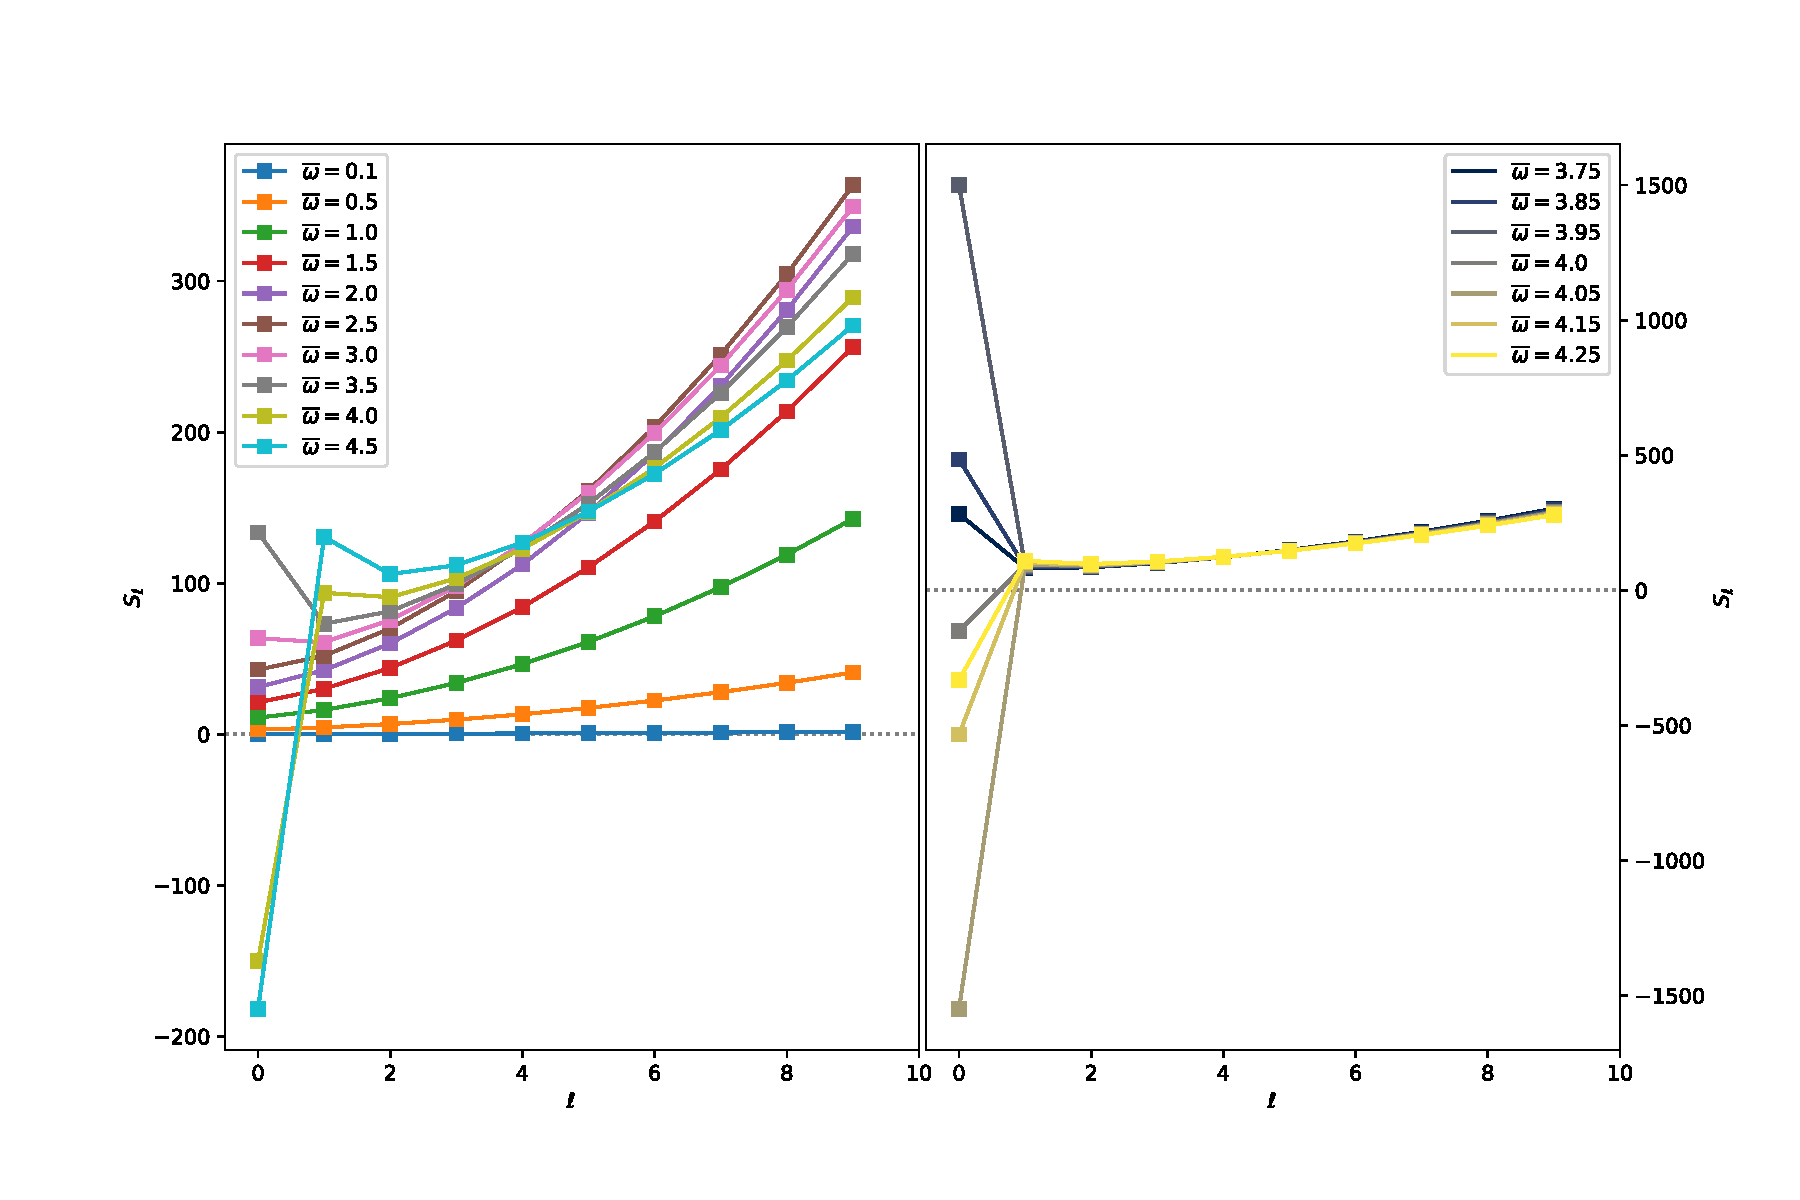
\includegraphics[width=\textwidth]{./figures/NN_equalfreq_sourceterms_m0_0+zoom}
\caption{{\it Left:} Evaluating $S_\ell$ (rescaled by the amplitudes) when $m^2 = 0$ for various choices of $\ob$. {\it Right}: The behaviour of $S_\ell$ for $\ob$ values near $\omega_0$.}
\label{fig:equal_frequency_m0}
\end{figure}

\begin{figure}[h]
\centering
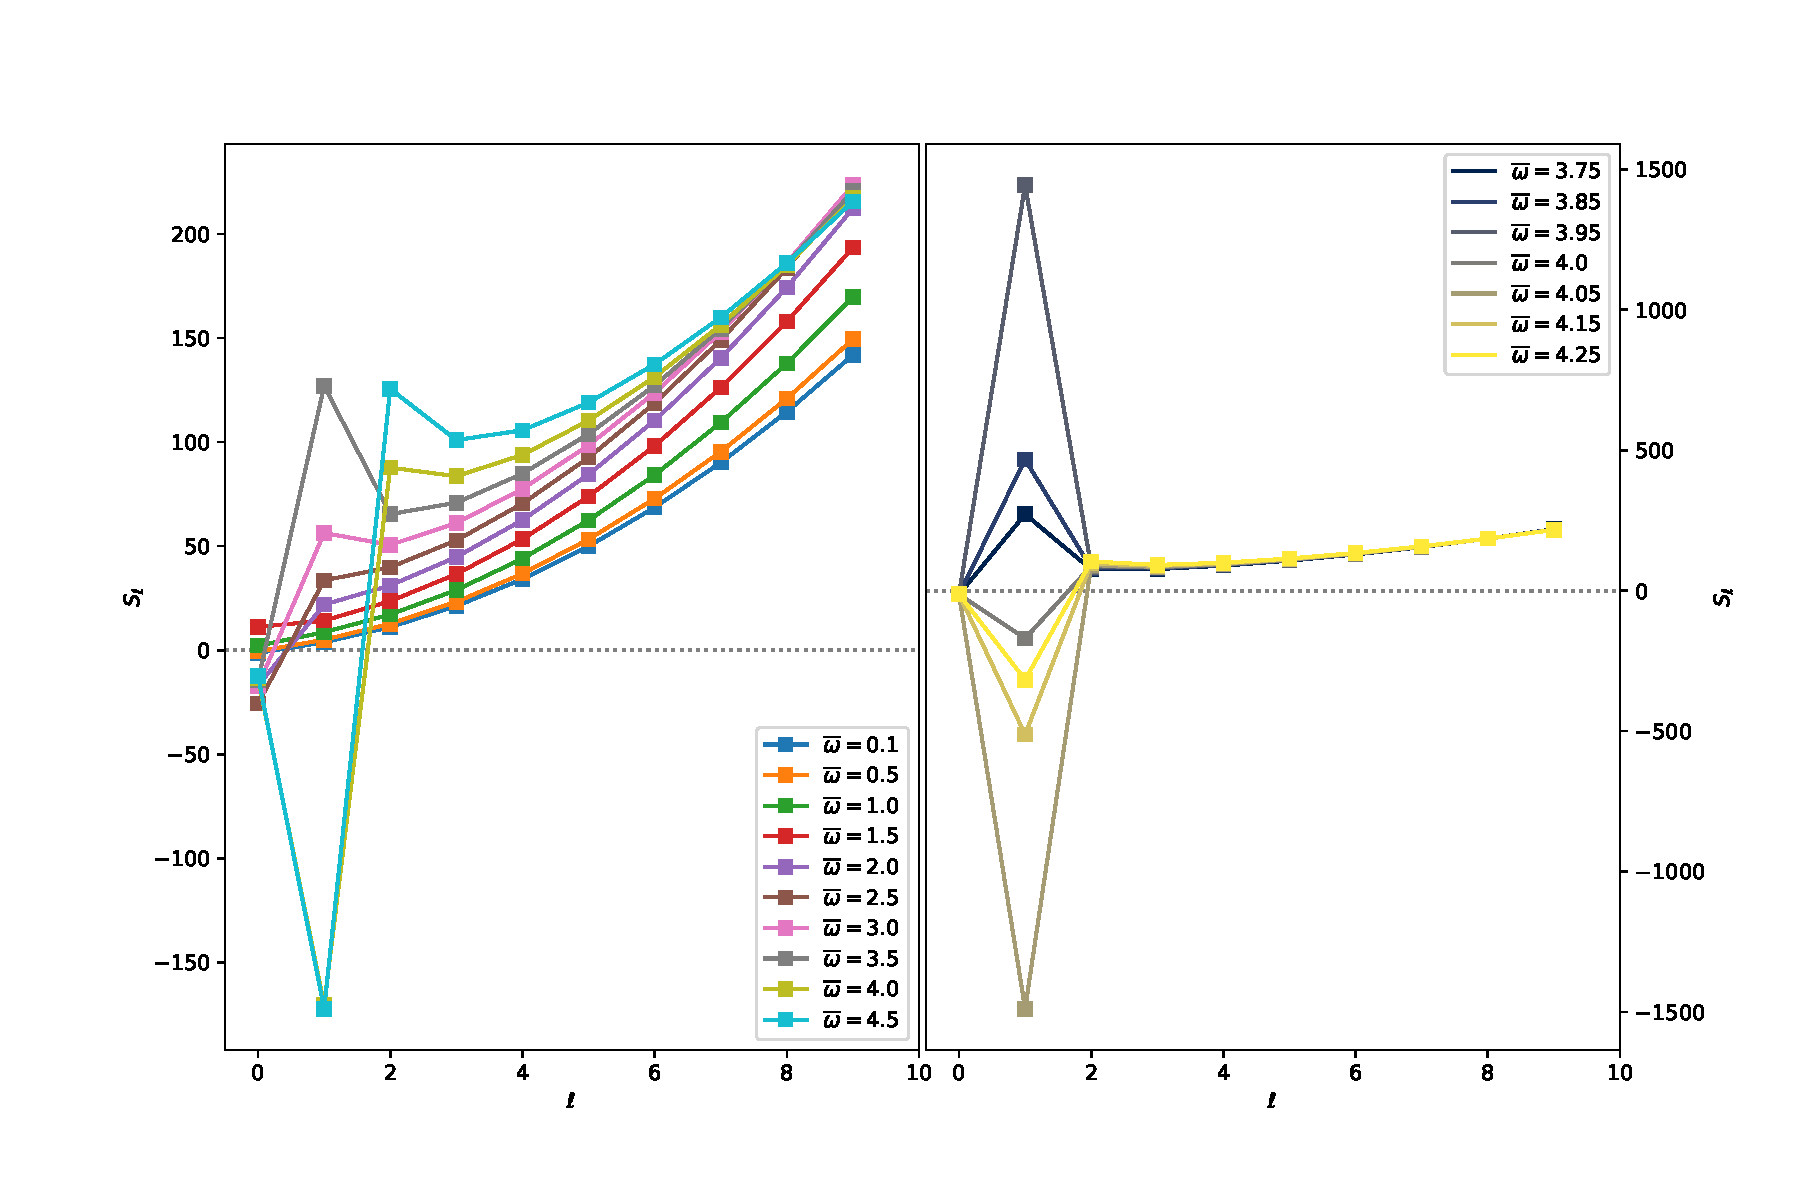
\includegraphics[width=\textwidth]{./figures/NN_equalfreq_sourceterms_m-4_0+zoom}
\caption{{\it Left:} Evaluating $\overline{T}_{\ell \ob}$ for a tachyon with $m^2 = -4.0$. {\it Right:} The behaviour of $S_\ell$ near $\omega_0 = \Delta^+ =  2$.}
\label{fig:equal_frequency_m-4_0}
\end{figure}

Other resonant contributions become possible for more restrictive values of the non-normalizable frequency, such as if $\ob$ is allow to be an integer. These contributions are not included here, but rather are discussed briefly in Appendix~\ref{more 2NN}.

\subsection{Special Values of Non-normalizable Frequencies}

Focus on non-arbitrary values of the non-normalizable frequencies.

\subsubsection{Add to an integer}
\label{ssec: add to integer}

Choose two of the modes to be non-normalizable with frequencies $\oone$ and $\otwo$ that add to give an integer: $\oone+ \otwo = 2n$ where $n = 1, 2, 3, \ldots$ (note that the $n = 0$ case means that both $\oone$ and $\otwo$ would need to be zero by the positive-frequency requirement and so would not contribute). Furthermore, either frequency need not be an integer and therefore the difference $|\oone - \otwo|$ will, in general, not be an integer. In \S\!~\ref{ssec: intpluschi}, we examine the case when the difference of non-normalizable frequencies is an integer.

When we consider possible resonance channels, we see that resonances can be grouped into
\begin{align}
\label{all pluses}
(++): \; \omega_i + 2n &= \omega_\ell \quad \forall \; \ell \geq n \\
(+-): \, \omega_i - 2n &=\omega_\ell \quad \forall \; n
\end{align}
for any $m^2_{BF} \leq m^2 < 0$. However, for a massless scalar, we have an additional channel
\begin{align}
\label{minus plus}
(-+): \, -\omega_i + 2n = \omega_\ell \quad \forall \; n \geq \ell + d
\end{align}
Adding the channels together, the total source term is
\begin{align}
\label{add to integer}
S_\ell &=   \overline{R}^{(+-)}_{(\ell + n) 1 2 \ell} \, \bar A_1 \bar A_2 \, a_{(\ell + n)} \cos\left( \theta_{(\ell + n)} - 2nt \right) + \overline{T}_{12\ell} \, \bar A_1 \bar A_2 \, a_\ell \cos \left( \theta_\ell \right) \nonumber \\ 
%
& \quad + \bigg[ \Theta\left( n - \ell - d \right) \overline{R}^{(-+)}_{(n - \ell - d) 1 2 \ell} \ \bar A_1 \bar A_2 \, a_{(n - \ell - d)} \cos \left( \theta_{(n - \ell - d)} - 2nt \right) \bigg]_{m^2 = 0} \nonumber \\
%
& \quad + \Theta \left( \ell - n \right)  \overline{R}^{(++)}_{(\ell - n) 1 2 \ell} \, \bar A_1 \bar A_2 \, a_{(\ell - n)} \cos \left( \theta_{(\ell - n)} + 2nt \right) ,
\end{align}
where the Heaviside step function $\Theta(x)$ enforces the restrictions on the indices in \eqref{all pluses} and \eqref{minus plus}. In the preceding expressions, the sum over all $\oone$, $\otwo$ such that $\oone + \otwo = 2n$ is implied, and only the restrictions on individual frequencies are included. Examining each channel in \eqref{add to integer} individually, we find
\begin{align}
\label{R1}
\overline{R}^{(++)}_{i 1 2 \ell} &= - \frac{1}{4} \sum_{\otwo \neq \ol} \frac{\otwo}{\ol - \otwo} Z^{-}_{i12\ell} - \frac{1}{4} \sum_{\oone \neq \ol} \frac{\oone}{\ol - \oone} Z^{-}_{i21\ell} - \frac{1}{8n} \sum \left( \ol - 2n \right) Z^-_{12i\ell} \nonumber \\
%
& - \frac{1}{4} \sum_{\oi \neq \oone} \frac{1}{\ol - \otwo} \Big[ \oone \left( H_{i12\ell} + m^2 V_{12i\ell} - 2 \otwo^2 X_{i12\ell} \right) + (\ol - 2n) \left( H_{1i2\ell} + m^2 V_{i21\ell} - 2\otwo^2 X_{1i2\ell} \right)\Big] \nonumber \\
%
& - \frac{1}{4} \sum_{\oi \neq \otwo} \frac{1}{\ol - \oone} \Big[ \otwo \left( H_{i21\ell} + m^2 V_{21i\ell} - 2\oone^2 X_{i21\ell} \right) + (\ol - 2n) \left( H_{2i1\ell} + m^2 V_{i12\ell} - 2\oone^2 X_{2i1\ell} \right) \Big] \nonumber \\
%
& - \frac{1}{8n} \sum_{\oone \neq \otwo} \Big[ \oone H_{21i\ell} + \otwo H_{12i\ell} + m^2 \left( \oone V_{1i2\ell} + \otwo V_{2i1\ell} \right) - \left( \ol - 2n \right)^2 \left(\oone X_{21i\ell} + \otwo X_{12i\ell} \right) \Big] \nonumber \\
%
& + \frac{1}{2} \sum \Big[ \oone\otwo X_{i12\ell} + \left( \ol - 2n \right)\left( \oone X_{21i\ell} + \otwo X_{12i\ell} \right) - \frac{m^2}{2} \left( V_{i12\ell} + V_{i21\ell} + V_{12i\ell} \right) \Big]
\end{align}
The notation $X_{i12\ell}$ corresponds to evaluating $X_{ijk\ell}$ with $\omega_j = \oone$ and $\omega_k = \otwo$. Next, we find that
\begin{align}
\label{R2}
\overline{R}_{i12\ell}^{(+-)} &= - \frac{1}{4} \sum \Big[ \frac{(\ol + 2n)}{2n} Z^-_{12i\ell} + 2 (\ol + 2n) \left( \oone X_{21i\ell} + \otwo X_{12i\ell} \right) \nonumber \\
%
& -\frac{\oone}{(\ol + \otwo)} \left( H_{i12\ell} + m^2 V_{12i\ell} - 2 \otwo^2 X_{i12\ell} \right) + \frac{(\ol + 2n)}{(\ol + \otwo)} \left( H_{1i2\ell} + m^2 V_{i21\ell} - 2\otwo^2 X_{1i2\ell} \right)  \nonumber \\
%
&- \frac{\otwo}{(\ol + \oone)} \left( H_{i21\ell} + m^2 V_{21i\ell} - 2\oone^2 X_{i21\ell} \right) + \frac{(\ol + 2n)}{(\ol + \oone)} \left(H_{2i1\ell} + m^2 V_{i12\ell} - 2\oone^2 X_{2i1\ell} \right)  \nonumber \\
%
&  - 2 \oone\otwo X_{i12\ell} + m^2 \left( V_{12i\ell} + V_{i12\ell} + V_{i21\ell} \right) \Big] + \frac{1}{4} \sum_{\otwo \neq \ol} \frac{\oone\otwo(\ol + 2n)}{\ol + \otwo} \left( X_{21i\ell} - X_{\ell i 12} \right) \nonumber \\
%
& + \frac{1}{4} \sum_{\oone \neq \ol} \frac{\oone\otwo(\ol + 2n)}{\ol + \oone} \left( X_{12i\ell} - X_{\ell i 12} \right).
\end{align}

When $m^2 = 0$, we have contributions from
\begin{align}
\label{R3}
\overline{R}_{i12\ell}^{(-+)} &=  \frac{1}{4} \sum_{\otwo \neq \ol} \frac{\otwo}{\ol - \otwo} Z^+_{i12\ell} + \frac{1}{4} \sum_{\oone \neq \ol} \frac{\oone}{\ol - \oone} Z^+_{i21\ell} + \frac{1}{4} \sum_{i \neq \ell} \left( \frac{2n - \ol}{2n} \right) Z^-_{12i\ell} \nonumber \\
%
& \quad + \frac{1}{4} \sum_{\oone \neq \oi} \frac{1}{\oi - \oone} \Big[ \oone \left( H_{i12\ell} - 2\otwo^2 X_{i12\ell} \right) - (2n - \ol) \left( H_{1i2\ell} - 2\otwo^2 X_{1i2\ell} \right) \Big] \nonumber \\
%
& \quad + \frac{1}{4} \sum_{\otwo \neq \oi} \frac{1}{\oi - \otwo} \Big[ \otwo \left( H_{i21\ell} - 2\oone^2 X_{i21\ell} \right) - (2n - \ol) \left( H_{2i1\ell} - 2\oone^2 X_{2i1\ell} \right) \Big] \nonumber \\
%
& \quad - \frac{1}{8n} \sum_{\oone \neq \otwo} \Big[ \oone H_{21i\ell} + \otwo H_{12i\ell} - 2 \left( 2n - \ol \right)^2 \left(\oone X_{21i\ell} + \otwo X_{12i\ell} \right) \Big] \nonumber \\
%
& \quad - \frac{1}{2} \sum \Big[ (2n - \ol) \left( \oone X_{21i\ell} + \otwo X_{12i\ell} \right) - \oone \otwo X_{i12\ell} \Big] .
\end{align}
{\it NB.}\, In \eqref{R3} \emph{only}, $\oi = 2i + \Delta^+ = 2i + d$ since this term requires that $m^2 = 0$ to contribute. We maintain the same notation out of convenience, despite the special case.

Finally, 
\begin{align}
\label{T12}
\overline{T}_{12\ell} &=  \frac{1}{2} \ol^2 \left( \tilde{Z}^+_{11\ell} + \tilde{Z}^+_{22\ell} \right)- \frac{1}{2} \Big[ H_{11\ell\ell} + H_{22\ell\ell} + m^2 \left( V_{\ell 1 1 \ell} + V_{\ell 2 2 \ell} \right) - 2 \ol^2 \left( X_{11\ell\ell} + X_{22\ell\ell} \right)  \nonumber \\
%
& \quad + 4 \ol^2 \left( \oone^2 P_{\ell \ell 1} + \otwo^2 P_{\ell \ell 2} \right) + 2\oone^2 M_{\ell \ell 1} + 2\otwo^2 M_{\ell \ell 2} + 2m^2 \left( \oone^2 Q_{\ell\ell 1} + \otwo^2 Q_{\ell \ell 2} \right) \Big] \, .
\end{align}

To examine the effect of the choice of $n$ on the value of $S_\ell$ and $| \Sigma S_\ell |$, figure~\ref{fig:atoi_all_m0_0compare} provides a comparison between the value of the source term for a massless scalar for two choices of $n$.

\begin{figure}
\centering
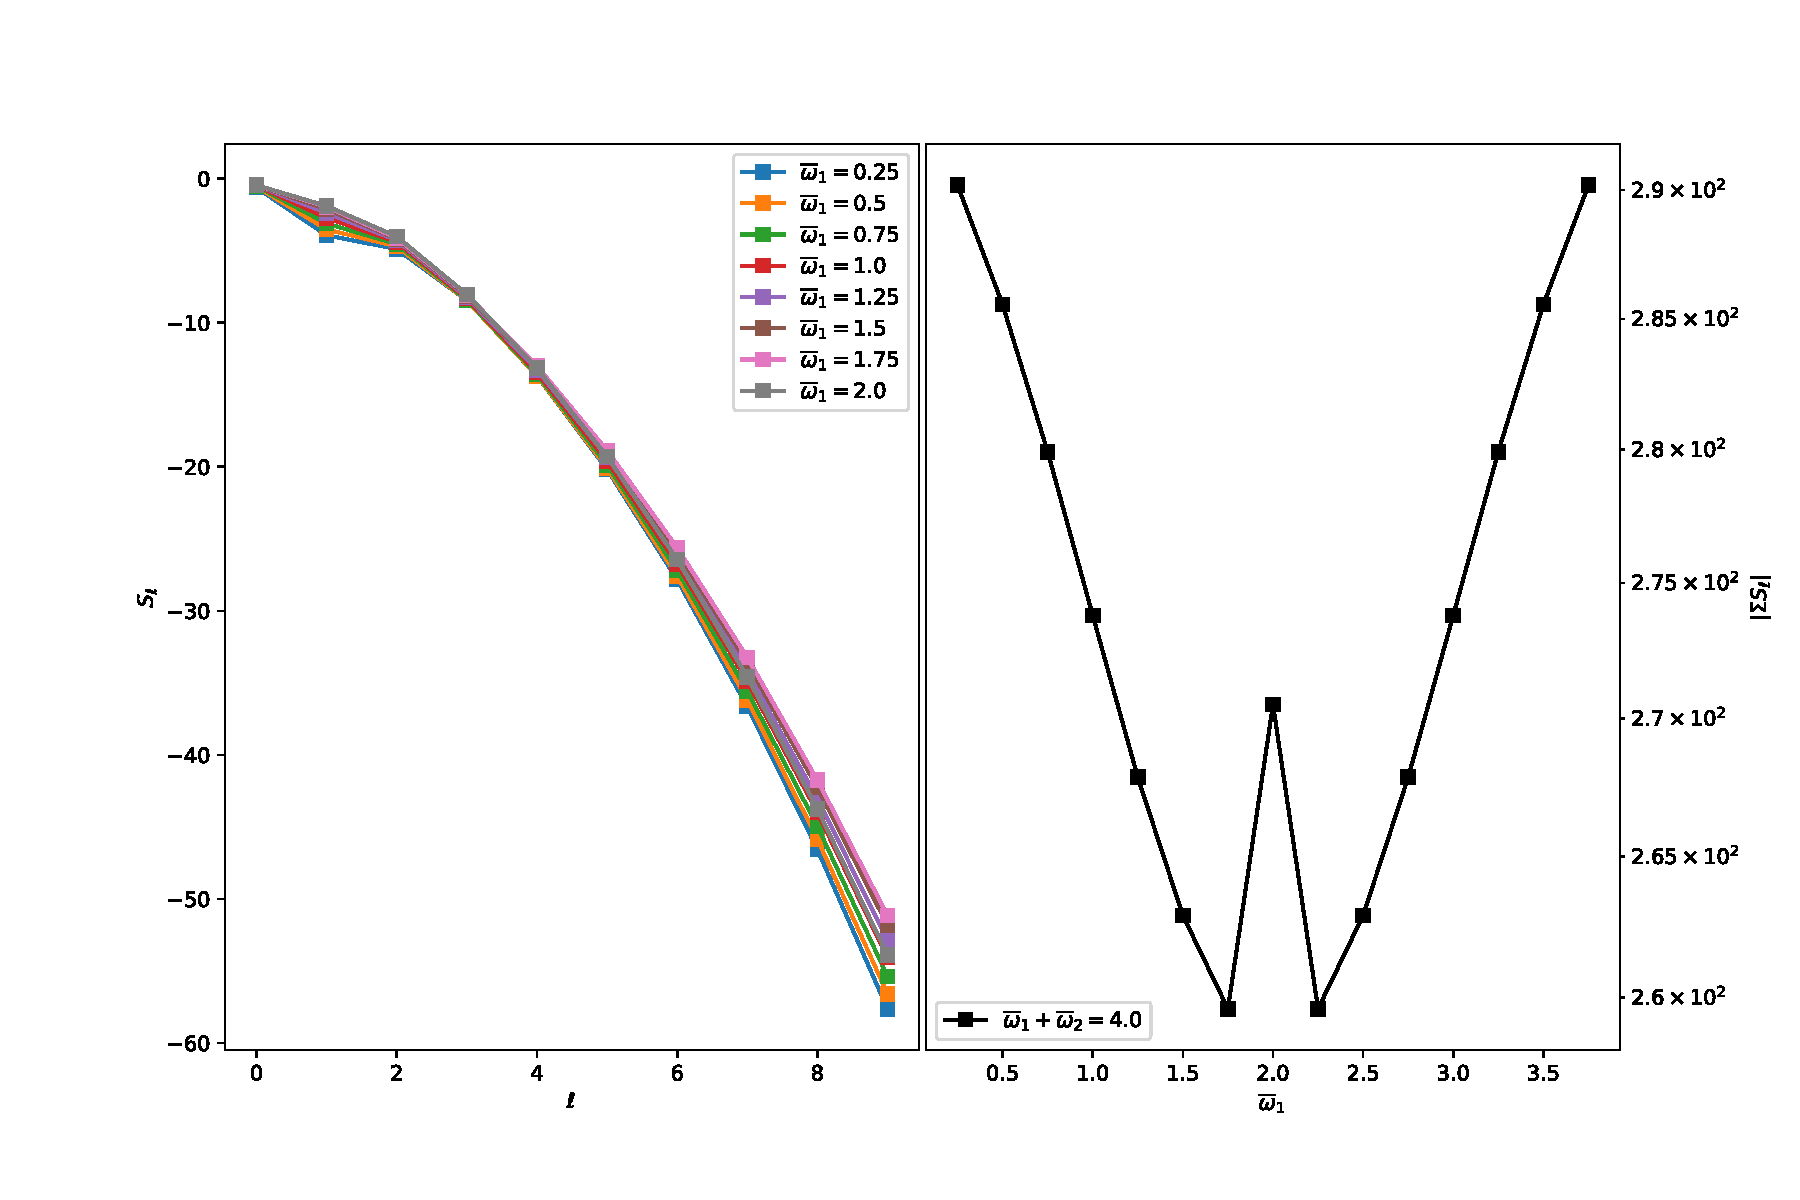
\includegraphics[width=\textwidth]{./figures/NNAddToInteger_source_n2_m-4_0}
\caption{{\it Left}: Source term values for a tachyonic scalar with $m^2 = -4.0$ when the frequencies of non-normalizable modes sum to $4.0$. {\it Right}: The absolute value of the sum of the source terms for each choice of $\oone$, $\otwo$.}
\label{fig:atoi_all_m-4_0}
\end{figure}

\begin{figure}[h!]
\centering
	\begin{subfigure}[b]{0.75\textwidth}
		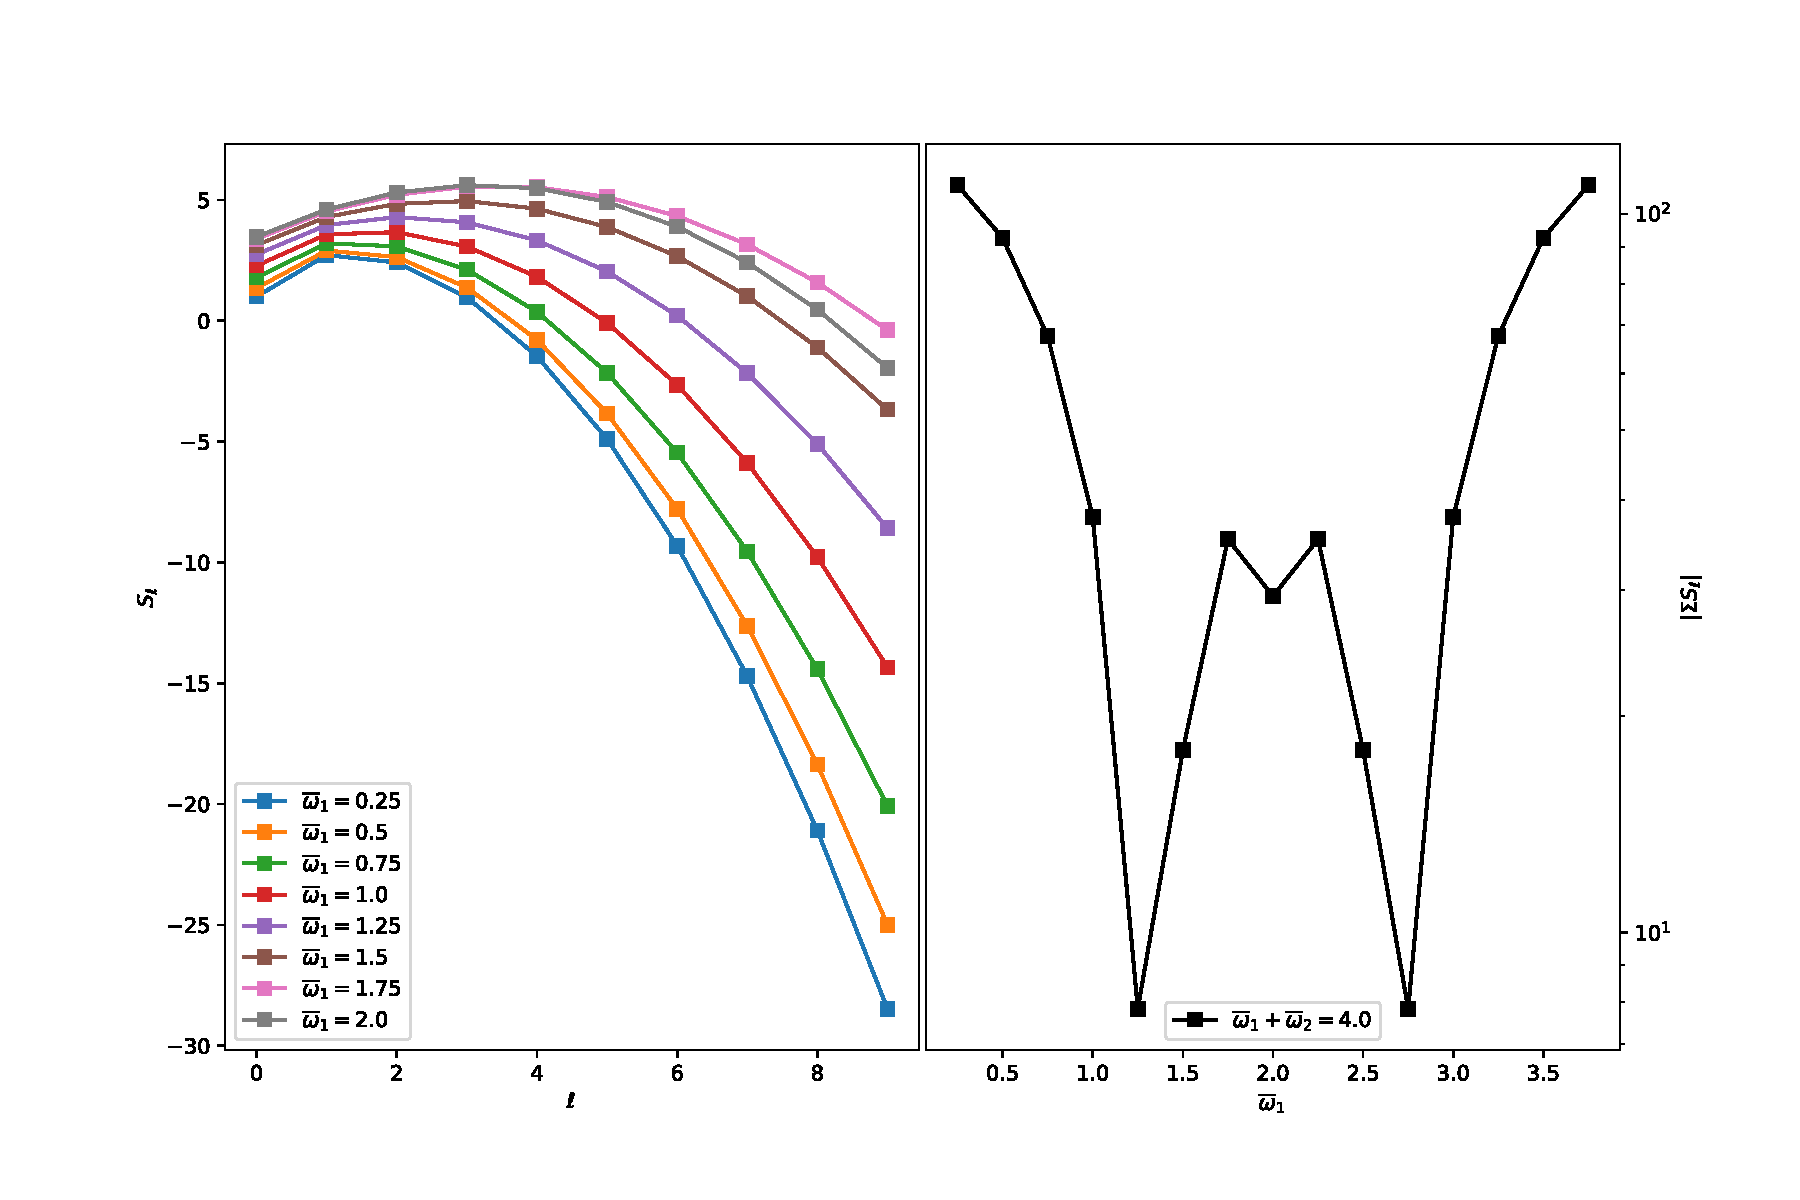
\includegraphics[width=\textwidth]{./figures/NNAddToInteger_source_n2_m0_0}
		\label{fig:atoi_all_n2_m0}
	\end{subfigure}
	\vspace{-0.25in}
	\begin{subfigure}[b]{0.75\textwidth}
		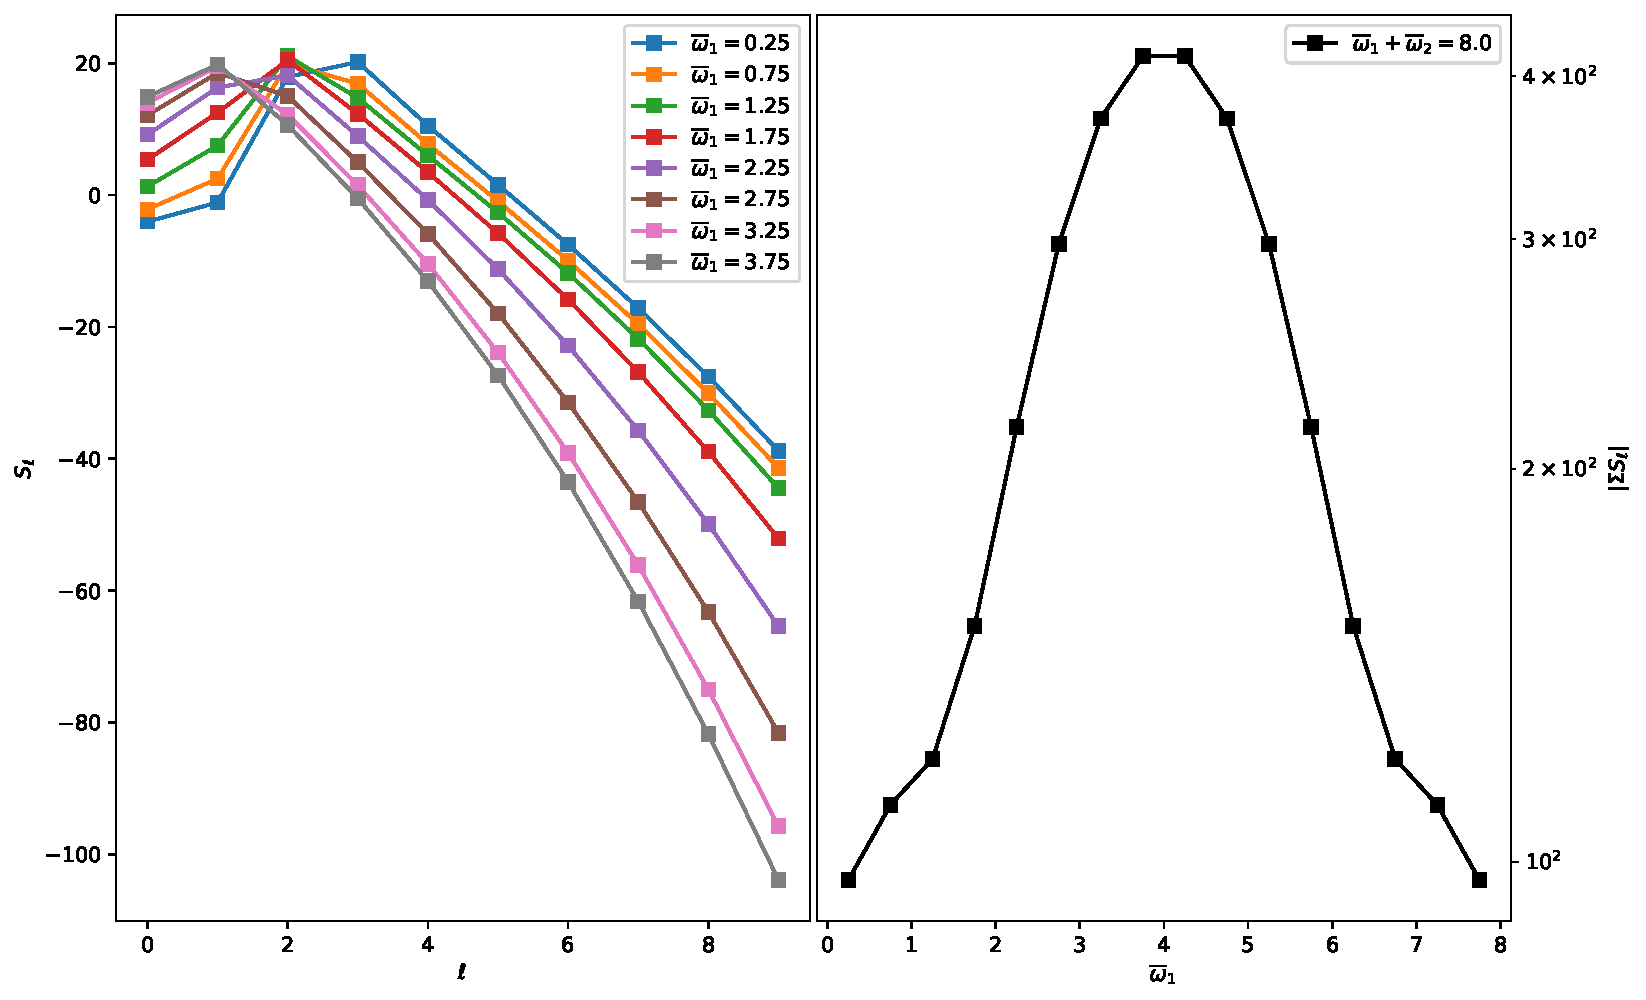
\includegraphics[width=\textwidth]{./figures/NNAddToInteger_source_n4_m0_0}
		\label{fig:atoi_all_n4_m0}
	\end{subfigure}
	\caption{{\it Above:} The value of \eqref{add to integer} as a function of $\ell$ for a massless scalar with values of $\oone$ and $\otwo$ chosen so that $\oone + \otwo = 4$. {\it Below:} The same plot but with values chosen to satisfy $\oone + \otwo = 8$.}
	\label{fig:atoi_all_m0_0compare}
\end{figure}

\subsection{Integer Plus $\chi$}
\label{ssec: intpluschi}

This is a case where the non-normalizable frequencies are non-integer, but differ from integer values by a specific amount. In analogue to the case where all modes are normalizable, we consider setting any two of the non-normalizable frequencies to
\begin{align}
\ogam = 2\gamma + \chi \, ,
\end{align}
where $m^2$ is \emph{not} chosen to be a special value\footnote{By tuning the value of the mass so that $\chi$ is an integer, additional resonant terms are possible; however, this scenario is addressed in \S\!~\ref{ssec: add to integer}. Furthermore, we do not consider the case when the Breitenlohmer-Freeman bound is saturated. This would place further restrictions on the allowed values of the indices in certain terms since the difference between the frequencies of normalizable and non-normalizable modes could then be zero.}, i.e. $\chi \notin \mathbb{Z}^*$, and $\gamma$ is an integer (greek letters are chosen to differentiate between normalizable modes with integer frequencies that use roman letters). For this choice of non-normalizable frequencies, there are no resonant contributions from the all-plus channel; only when either $\oi + \ogam = \obet - \ol$, or $\oi + \ogam = \obet + \ol$ with $i + \gamma \geq \ell$, are resonant terms present.

\subsubsection{$\oi + \ogam = \obet - \ol$}
\label{sssec: intpluschi1}

This channel contributes secular terms of the form
\begin{align}
\label{intpluschi1 source}
S_\ell &= \sum_{i \neq \ell} \sum_{\gamma \neq \beta} \overline{S}_{i (i + \gamma + \ell) \gamma \ell} \cos \left( \theta_i - \theta_{(i + \gamma + \ell)} + \theta_\gamma \right) + \sum_\beta \overline{R}_{\beta \ell} \cos \left(\theta_\ell + \theta_\beta - \theta_\beta \right) 
\end{align}
where 
\begin{align}
\overline{S}_{i \beta\gamma\ell} &= \frac{1}{4} H_{\beta\gamma i \ell} \frac{ \ogam (\oi - \obet + 2\ogam)}{(\obet - \ogam)(\oi + \ogam)} - \frac{1}{4} H_{\gamma\beta i \ell} \frac{\obet(\oi + \ogam - 2\obet)}{(\oi - \obet)(\obet - \ogam)} - \frac{1}{4} H_{\gamma i \beta\ell} \frac{\oi (\ogam - \obet + 2\oi)}{(\oi - \obet)(\oi + \ogam)} \nonumber \\
%
& + \frac{1}{2} \oi \ogam X_{\beta\gamma i \ell} \left( \frac{\ogam}{\oi - \obet} - \frac{\oi}{\obet + \ogam} + 1 \right) + \frac{1}{2} \oi \obet X_{\gamma\beta i \ell} \left( \frac{\oi}{\obet - \ogam} + \frac{\obet}{\oi + \ogam} - 1 \right) \nonumber \\
%
& + \frac{1}{2} \obet \ogam X_{i\beta\gamma\ell} \left(\frac{\obet}{\oi + \ogam} - \frac{\ogam}{\oi - \obet} - 1 \right) - \frac{1}{4} Z^+_{\beta\gamma i \ell} \left( \frac{\oi}{\oi + \ol}\right)  \nonumber \\
%
& + \frac{1}{4} Z^{-}_{i\gamma\beta\ell} \left(  \frac{\obet}{\ol - \obet}  \right) + \frac{1}{4} Z^+_{i\beta\gamma\ell} \left( \frac{\ogam}{\ol + \ogam} \right)
\end{align}
and
\begin{align}
\overline{R}_{\beta \ell} &= \frac{1}{4} Z^{-}_{\ell \beta \beta \ell} \left( \frac{\obet}{\ol + \obet} \right) +  \frac{1}{4} Z^+_{\ell \beta \beta \ell} \left(\frac{\obet}{\ol - \obet} \right) + \frac{1}{2} H_{\ell\beta\beta\ell} \left( \frac{\obet^2}{\ol^2 - \obet^2} \right) - \frac{1}{2} H_{\beta \ell\beta\ell} \left( \frac{\ol^2}{\ol^2 - \obet^2} \right) \nonumber \\
%
& + X_{\beta\ell\beta\ell} \left( \frac{\ol^4}{\ol^2 - \obet^2} \right)  - \frac{1}{2} \obet^2  X_{\ell\beta\beta\ell} \left(\frac{\ol^2 + \obet^2 }{\ol^2 - \obet^2} \right)  - \frac{1}{2} H_{\ell\beta\beta\ell} + \ol^2 \tilde{Z}^+_{\beta\beta\ell} -2 \obet^2 \ol^2 P_{\ell\ell\beta} - \obet^2 M_{\ell\ell\beta}
\end{align}

\subsubsection{$\oi + \ogam = \obet + \ol$}
\label{ssec: intpluschi2}

This channel contributes secular terms of the form
\begin{align}
\label{intpluschi2 source}
S_\ell = \underbrace{\sum_{i \neq \ell} \sum_{\gamma \neq \beta}}_{i + \gamma \geq \ell} \overline{S}_{i (i + \gamma - \ell) \gamma \ell} \cos \left( \theta_i - \theta_{(i + \gamma - \ell)} + \theta_\gamma \right) + \sum_\beta \overline{R}_{\beta\ell} \cos \left( \theta_\ell + \theta_\beta - \theta_\beta \right)
\end{align}
where
\begin{align}
\overline{S}_{i\beta\gamma\ell} &= \frac{1}{4} H_{\beta\gamma i\ell} \frac{\ogam (\oi - \obet)}{(\obet - \ogam)(\oi - \ogam)} - \frac{1}{4} H_{\gamma\beta i \ell} \frac{\obet(\ol - \obet)}{(\obet - \ogam)(\oi - \obet)} + \frac{1}{4} H_{\beta i \gamma\ell} \frac{\oi (\ogam - \obet)}{(\oi - \obet)(\oi - \ogam)} \nonumber \\
%
& + \frac{1}{2} \oi \ogam X_{\beta\gamma i \ell} \left( \frac{\ogam}{\oi - \obet} - \frac{\oi}{\obet - \ogam} + 1 \right) + \frac{1}{2} \oi \obet X_{\gamma\beta i \ell} \left( \frac{\oi}{\obet - \ogam} - \frac{\obet}{\oi - \ogam} - 1 \right) \nonumber \\
%
& + \frac{1}{2} \obet \ogam X_{i\beta\gamma\ell} \left( \frac{\obet}{\oi - \ogam} - \frac{\ogam}{\oi - \obet} - 1 \right)  + \frac{1}{4} Z^-_{i\gamma\beta\ell} \left( \frac{\obet}{\ol + \obet}\right)  \nonumber \\
%
&
+ \frac{1}{4} Z^+_{i\beta\gamma\ell} \left( \frac{\ogam}{\ol - \ogam}\right) - \frac{1}{4}Z^+_{\beta\gamma i \ell} \left( \frac{\oi}{\oi - \ol} \right) 
\end{align}
and
\begin{align}
\overline{R}_{\beta\ell} &= \frac{1}{4} Z^-_{\ell\beta\beta\ell} \left( \frac{\obet}{\ol + \obet} \right) + \frac{1}{4} Z^+_{\ell\beta\beta\ell} \left( \frac{\obet}{\ol - \obet} \right) + \frac{1}{2} H_{\ell\beta\beta\ell} \left( \frac{\obet^2}{\ol^2 - \obet^2} \right) - \frac{1}{2} H_{\beta\ell\beta\ell} \left( \frac{\ol^2}{\ol^2 - \obet^2} \right) \nonumber \\
%
& \!\!\!\!\!\!\!\! + X_{\beta\beta\ell\ell} \left( \frac{\ol^2}{\ol^2 - \obet^2} \right) + \frac{1}{2} \obet^2 X_{\ell\beta\beta\ell} \left( \frac{\ol^2 + \obet^2}{\ol^2 - \obet^2} \right) - \frac{1}{2} H_{\beta\beta\ell\ell} +  \ol^2 \tilde{Z}^+_{\beta\beta\ell} - 2 \obet^2 \ol^2 P_{\ell\ell\beta} - \obet^2 M_{\ell\ell\beta} \vspace{-0.3in}
\end{align}

\begin{figure}[h!]
\centering
	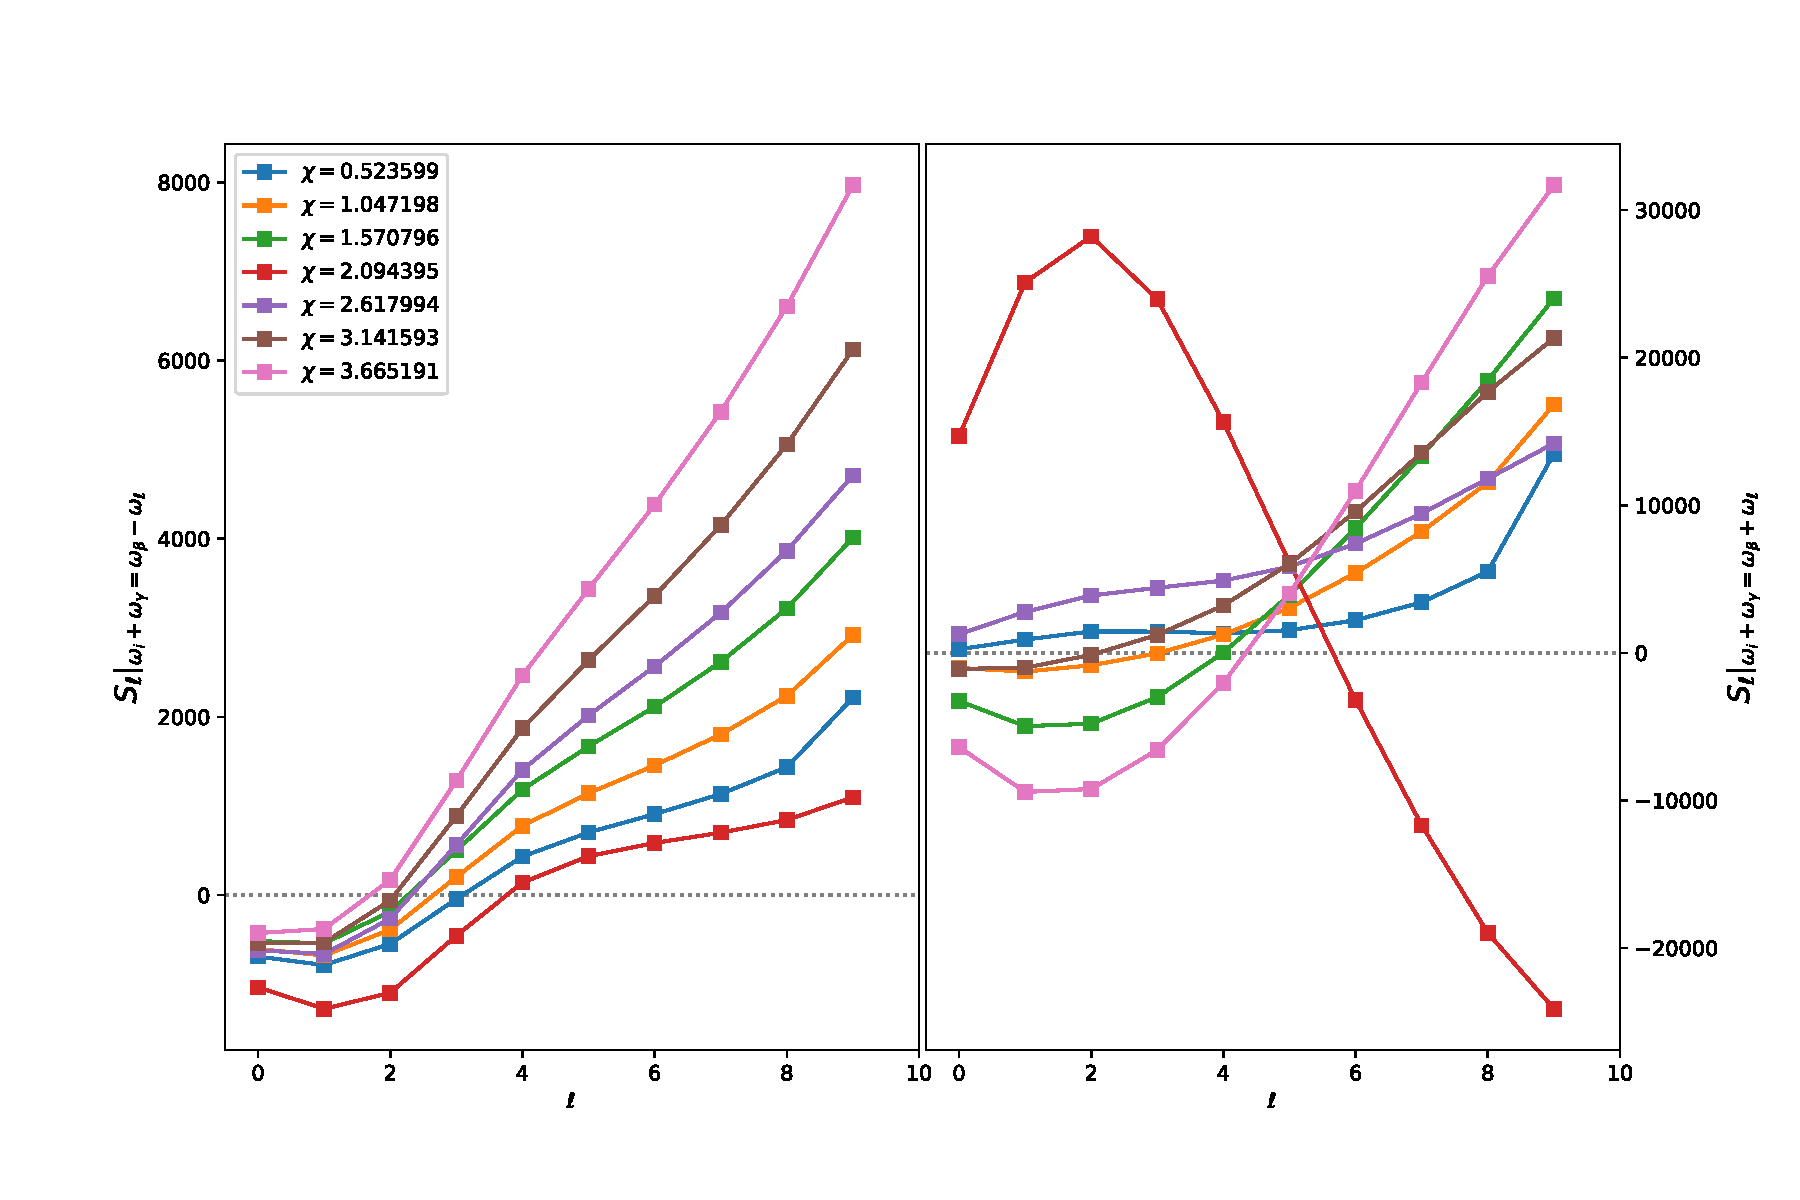
\includegraphics[width=\textwidth]{./figures/IntPlusChi}
	\caption{{\it Left:} Evaluating the source term \eqref{intpluschi1 source} for various values of $\chi$ for $\ell < 10$. {\it Right:} Evaluating the source term \eqref{intpluschi2 source} subject to $i + \gamma \geq \ell$ for the same values of $\chi$ and the same range of $\ell$.}
	\label{fig: twoiplusx}
\end{figure}

In figure~\ref{fig: twoiplusx}, we evaluate both resonance channels and plot their contributions for various values of $\chi$. In particular, we examine values $\chi \in \{ \pi/6, \ldots, 7\pi/6 \}$.


%%%%%%%%%%%%%%%%%%%%%%%%%%%%%%%%%%%%%%%%%
%%%%%%%%%%%%%%%%%%%%%%%%%%%%%%%%%%%%%%%%%

\section{Discussion}
\label{sec: discussion}

Discussion goes here.

%%%%%%%%%%%%%%%%%%%%%%%%%%%%%%%%%%%%%%%%%
%%%%%%%%%%%%%%%%%%%%%%%%%%%%%%%%%%%%%%%%%

%\acknowledgments

%%%%%%%%%%%%%%%%%%%%%%%%%%%%%%%%%%%%%%%%%
%%%%%%%%%%%%%%%%%%%%%%%%%%%%%%%%%%%%%%%%%

\appendix
\section{Derivation of Source Terms For Massive Scalars}
\label{app: source term derivation}

The backreaction between the metric and the scalar field appears at second order in the perturbation,
\begin{align}
A_2' = - \mu \nu \left[ (\dot \phi_1 )^2 + (\phi_1')^2 + m^2 \phi_1^2 \sec^2 x \right] + \nu' A_2 / \nu
\end{align}
which can be directly integrated to give

\begin{align}
A_2 = -\nu \int^x_0 dy \, \mu \left( (\dot \phi_1 )^2 + (\phi_1')^2 + m^2 \phi_1^2 \sec^2 x \right) \, .
\end{align}
Furthermore, the first non-trivial contribution to the lapse in the boundary time gauge is

\begin{align}
\delta_2 = \int^{\pi/2}_x dy \, \mu \nu \left(  (\dot \phi_1 )^2 + (\phi_1')^2 \right) \, .
\end{align}
For convenience, we have also defined the functions
\begin{align}
\mu (x) = \left( \tan x \right)^{d-1} \quad \text{and} \quad \nu(x) = (d-1) / \mu ' \, .
\end{align}

To aide in evaluating integrals, we first derive the following identities: from the equation for the first-order time-dependent coefficients $c_i$,
\begin{align} 
\ddot c_i + \oi^2 c_i = 0 \quad \Rightarrow \quad \p_t \left(\dot c_i^2 + \oi^2 c_i^2 \right) = \p_t \mathbb C_i = 0 \, ;
\end{align}
from the equation definition of $\hat L$,
\begin{align}
\hat L e_j = -\frac{1}{\mu} \left( \mu e'_j \right)' + m^2 \sec^2 x e_j \quad \Rightarrow \quad \left( \mu e'_j \right)' = \mu \left( m^2 \sec^2 x - \omega_j^2 \right) e_j \, ;
\end{align}
from considering the expression $\left( \mu e'_i e_j \right)'$:
\begin{align}
\left( \mu e'_i e_j \right) ' = \left(m^2 \sec^2 x - \oi^2 \right) \mu e_i e_j + \mu e'_i e'_j \, ;
\end{align}
from permuting $i, j$ above and subtracting to give
\begin{align}
\frac{\left[ \mu (e'_i e_j \oj^2 - e_i e'_j \oi^2 ) \right]'}{(\oj^2 - \oi^2)} = \mu m^2 \sec^2 x e_i e_j + \mu e'_i e'_j \, .
\end{align}


The derivation of the source terms for massive scalars closely follows the massless case, particularly if one chooses not to write out the explicit mass dependence as was done in \cite{1810.04753}. However, since we have chosen to write our equations in a slightly different way -- and in a different gauge -- than previous authors, one may find it instructive to see the differences in the derivations. Below we have included the intermediate steps involved in deriving the third-order source term $S_\ell$.

Projecting each of the terms individually onto the eigenbasis $\{ e_\ell \}$:
\begin{align}
\langle \delta_2 \ddot \phi_1, e_\ell \rangle &= - \sum_{i = 0}^\infty \sum_{\substack{j=0 \\ k \neq \ell}}^\infty \sum_{k=0}^\infty \frac{\ok^2 c_k}{\ol^2 - \ok^2} \left[\dot c_i \dot c_j \left(X_{k\ell ij} - X_{\ell k i j} \right) + c_i c_j \left( Y_{ij\ell k} - Y_{ijk\ell} \right) \right] \nonumber \\
& \qquad  - \sum_{i=0}^\infty \sum_{j=0}^\infty \ol^2 c_\ell \left[ \dot c_i \dot c_j P_{ij\ell} + c_i c_j B_{i j \ell} \right] \, , \\
%
\langle A_2 \ddot \phi_1, e_\ell \rangle &= 2 \sum_{i = 0}^\infty \sum_{\substack{j=0 \\ i \neq j}}^\infty \sum_{k=0}^\infty \frac{\ok^2 c_k}{\oj^2 - \oi^2} X_{ijk \ell} \left( \dot c_i \dot c_j + \oj^2 c_i c_j \right) \nonumber \\
& \qquad + \sum_{i = 0}^\infty \sum_{j = 0}^\infty \oj^2 c_j \left( \mathbb C_i P_{j \ell i} + c_i^2 X_{ii j \ell} \right) \, , \\
%
\langle \dot \delta_2 \dot \phi_1 , e_\ell \rangle &= \sum_{i = 0}^\infty \sum_{\substack{j=0 \\ k \neq \ell}}^\infty \sum_{k=0}^\infty \frac{\dot c_k}{\ol^2 - \ok^2} \left[ \p_t \left( \dot c_i \dot c_j \right) \left( X_{k\ell ij} - X_{\ell k i j} \right) + \p_t (c_i c_j) \left(Y_{ij\ell k} - Y_{ijk\ell}\right) \right] \nonumber \\
& \qquad+ \sum_{i=0}^\infty \sum_{j=0}^\infty \dot c_\ell \left[ \p_t \left( \dot c_i \dot c_j \right) P_{ij\ell} + \p_t (c_i c_j) B_{ij\ell} \right] \, , \\
%
\langle \dot A_2 \dot \phi_1, e_\ell \rangle &= -2 \sum_{i=0}^\infty \sum_{j=0}^\infty \sum_{k=0}^\infty  \dot c_k \dot c_j c_i X_{ijk\ell} \, , \\
%
\langle \left( A_2' - \delta_2' \right) \phi_1', e_\ell \rangle &= - 2 \sum_{i = 0}^\infty \sum_{\substack{j=0 \\ i \neq j}}^\infty \sum_{k=0}^\infty \frac{c_k (\dot c_i \dot c_j + \oj^2 c_i c_j)}{\oj^2 -\oi^2} H_{ijk\ell} -m^2 \sum_{i=0}^\infty \sum _{j=0}^\infty \sum_{k=0}^\infty c_i c_j c_k V_{ijk\ell} \nonumber \\
%
& \qquad - \sum_{i=0}^\infty \sum_{j=0}^\infty c_j \left[ c_i^2 H_{iij\ell} + \mathbb C_i M_{j \ell i} \right] \, , \\
%
\langle A_2 \phi_1 \sec^2 x, e_\ell \rangle &= - 2\sum_{i = 0}^\infty \sum_{\substack{j=0 \\ i \neq j}}^\infty \sum_{k=0}^\infty \frac{c_k (\dot c_i \dot c_j + \oj^2 c_i c_j )}{\oj^2 - \oi^2} V_{jki\ell} \nonumber \\
& \qquad - \sum_{i=0}^\infty \sum_{j=0}^\infty c_j \left( c_i^2 V_{jii\ell} + \mathbb C_i Q_{j\ell i} \right) .
\end{align}

Where the forms of X, Y, V, H, B, M, P, and Q are given by
\begin{align}
X_{ijk\ell} &= \int^{\pi/2}_0 dx \, \mu^2 \nu e'_i e_j e_k e_\ell \\
Y_{ijk\ell} &= \int^{\pi/2}_0 dx \, \mu^2 \nu e'_i e'_j e_k e'_\ell \\
V_{ijk\ell} &= \int^{\pi/2}_0 dx \, \mu^2 \nu e_i e_j e'_k e_\ell \sec^2 x \\
H_{ijk\ell} &= \int^{\pi/2}_0 dx \, \mu^2 \nu' e'_i e_j e'_k e_\ell \\
B_{ij\ell} &= \int^{\pi/2}_0 dx \, \mu \nu e'_i e'_j \int^x_0 dy \, \mu e^2_\ell \\
M_{ij\ell} &= \int^{\pi/2}_0 dx \, \mu \nu' e'_i e_j \int^x_o dy \, \mu e_\ell^2 \\
P_{ij\ell} &= \int^{\pi/2}_0 dx \, \mu \nu e_i e_j \int^x_0 dy \, \mu e^2_\ell \\
Q_{ij\ell} &= \int^{\pi/2}_0 dx \, \mu \nu e_i e_j \sec^2 x \int^x_0 dy \, \mu e^2_\ell
\end{align}

Collecting terms together gives the expression for $S_\ell = \langle S, e_\ell \rangle$:
\begin{align}
S_\ell &= \sum_{\substack{i, j, k \\ k \neq \ell}}^\infty \frac{1}{\ol^2 - \ok^2} \Big[ F_k(\dot c_i \dot c_j) \left(X_{k\ell i j} - X_{\ell k i j} \right) + F_k(c_i c_j) \left(Y_{ij\ell k} - Y_{ijk\ell} \right) \Big] \nonumber \\
%
& \quad +2 \sum_{\substack{i,j,k \\ i \neq j}}^\infty \frac{c_k D_{ij}}{\oj^2 - \oi^2} \Big[  2\ok^2 X_{ijk\ell} - H_{ijk\ell} -m^2 V_{jki\ell} \Big] - \sum_{i,j,k}^\infty c_i \Big[ 2 \dot c_j \dot c_k X_{ijk\ell} + m^2 c_j c_k V_{ijk\ell} \Big] \nonumber \\ 
%
& \quad + \sum_{i,j}^\infty \Big[ F_\ell (\dot c_i \dot c_j) P_{ij\ell} + F_\ell (c_i c_j) B_{ij\ell} + 2\oj^2 c_j \left( c_i^2 X_{iij\ell} + \mathbb C_i P_{j\ell i} \right) \nonumber \\
%
& \qquad - c_j \left( c^2_i (H_{iij\ell} + m^2 V_{jii\ell} ) + \mathbb C_i (M_{j\ell i} + m^2 Q_{j\ell i}) \right) \Big] \, ,
\end{align}
where $F_k(z) = \dot c_k \dot z - 2\ok^2 c_k z$, $D_{ij} = \dot c_i \dot c_j + \omega^2_j c_i c_j$, and $\mathbb C_i = \dot c_i^2 + \oi^2 c_i^2$.

To simplify the above expression, we have defined
\begin{align}
Z^{\pm}_{ijk\ell} = \oi \oj \left( X_{k\ell ij} - X_{\ell kij} \right) \pm \left( Y_{ij\ell k} - Y_{ijk\ell} \right) \quad \text{and} \quad \tilde Z^{\pm}_{ij\ell} = \oi \oj P_{ij\ell} \pm B_{ij\ell} \, .
\end{align}

Using integration by parts to remove the derivative from $\nu$ in the definitions of $H_{ijk\ell}$ and $M_{ij\ell}$, we can show that
\begin{align}
H_{ijk\ell} &= \oi^2 X_{kij\ell} + \ok^2 X_{ijk\ell} - Y_{ij\ell k}  - Y_{\ell kji}   - m^2 V_{kji\ell} -m^2 V_{ijk\ell} \\
M_{ij\ell} &= \oi^2 P_{ij\ell} - B_{ij\ell} -m^2 Q_{ij\ell}
\end{align}

\section{Two Non-normalizable Modes with Equal Frequencies}
\label{more 2NN}
Let us return to the case of two, equal, non-normalizable modes with frequency $\ob$. Within the space of resonant frequency values, there are frequencies that happen to satisfy $\ob = \ol$ numerically and may produce extra resonances subject to restrictions on the normalizable frequency. These instances were excluded from the discussion in \S\!~\ref{ssec: equalNN}, and we address them here. When considering special integer values of $\ob$ each choice of $\ob$ below will contribute a $\overline T$-type term to the total source:
\begin{align}
\label{gen NN res 1}
\overline{T}^{(1)}_{i}: \quad \omega_i &= \ol + 2\ob \quad \forall \; \ob \in \mathbb{Z}^* \\
\overline{T}^{(2)}_{i}: \quad \omega_i &= \ol - 2\ob \quad \forall \; \ob \in \mathbb{Z}^* \; \text{such that } \ell \geq \ob \\
\label{gen NN res 2}
\overline{T}^{(3)}_{i}: \quad \omega_i &= 2\ob - \ol \quad \forall \; \ob \in \mathbb{Z}^* \; \text{such that } \ob \leq \ell + \Delta^+ \, ,
\end{align}
with $\omega_i \neq \omega_\ell$ in each case. These special values contribute to the case of two, equal non-normalizable modes via
\begin{align}
\label{2NN all}
S_\ell &= \bar A^2_{\ob} \, \overline{T}^{(1)}_{(\ell + \ob)} \, a_{(\ell + \ob)} \cos \left( \theta_{(\ell + \ob)} - 2\ob t \right) + \bar A^2_{\ob} \, \overline{T}^{(2)}_{(\ell - \ob)} \, a_{(\ell - \ob)}\cos \left( \theta_{(\ell - \ob)} + 2\ob t \right) \nonumber \\
& \quad + \bar A^2_{\ob} \, \overline{T}^{(3)}_{(\ob - \ell - \Delta^+)} \, a_{(\ob - \ell- \Delta^+)} \cos \left( 2\ob t - \theta_{(\ob - \ell - \Delta^+)} \right) 
\end{align}
under their respective conditions on the value of $\ob$. The total resonant contribution for all possible $\ob$ values is the addition of \eqref{2NN all} and \eqref{2genNN}. 
Evaluating \eqref{general source} in each case of the cases described by \eqref{gen NN res 1}~\!-~\!\eqref{gen NN res 2}, we find that
\begin{align}
\overline{T}^{(1)}_{i} &= \frac{1}{2} \bigg[ \, H_{i\ob\ob\ell} \left( \frac{\ob}{\oi - \ob} \right) - H_{\ob i \ob\ell} \left( \frac{\oi}{\oi - \ob} \right) + m^2 V_{\ob\ob i\ell} \left( \frac{\ob}{\oi - \ob} \right) \nonumber \\
%
& - m^2 V_{i \ob\ob\ell} \left( \frac{\oi}{\oi - \ob} \right) - 2 \ob^2 X_{i\ob\ob\ell} \left( \frac{\ob}{\oi - \ob} \right) + 2 \ob^2 X_{\ob i \ob\ell} \left( \frac{\oi}{\oi - \ob} \right) \bigg]_{\oi \neq \ob} \nonumber \\
%
& -\frac{1}{2} \bigg[ Z^+_{i\ob\ob\ell} \left( \frac{\ob}{\ol + \ob} \right) \bigg]_{\ol \neq \ob} \!\! + \frac{1}{4} Z^-_{\ob\ob i \ell} \left( \frac{\ol + 2\ob}{2 \ob} \right) + \frac{1}{2} \ob^2 X_{i\ob\ob\ell} - \frac{m^2}{4} V_{\ob\ob i \ell} \nonumber \\
%
& - \ob \oi X_{\ob\ob i\ell} - \frac{m^2}{2} V_{i \ob\ob\ell} \, ,
\end{align}
\begin{align}
\overline{T}^{(2)}_{i} &=  - \frac{1}{2} \bigg[ \, H_{i\ob\ob \ell} \left( \frac{\ob}{\oi + \ob} \right) + H_{\ob i \ob \ell} \left( \frac{\oi}{\oi + \ob} \right) + m^2 V_{\ob \ob i \ell} \left( \frac{\ob}{\oi + \ob} \right) \nonumber \\
%
& + m^2 V_{i\ob\ob\ell} \left( \frac{\oi}{\oi + \ob} \right) - 2 \ob^2 X_{i \ob\ob\ell} \left( \frac{\ob}{\oi + \ob} \right) - 2 \ob^2 X_{\ob\ob i\ell} \left( \frac{\oi}{\oi + \ob} \right) \bigg]_{\oi \neq \ob} \nonumber \\
%
& - \frac{1}{2} \bigg[ \, Z^{-}_{i \ob \ob \ell} \left( \frac{\ob}{\ol - \ob} \right) \bigg]_{\ol \neq \ob} \!\!\!\! - \frac{1}{4} Z^-_{\ob\ob i \ell} \left( \frac{\ol - 2\ob}{\ob} \right) + \frac{1}{2} \ob^2 X_{i\ob\ob\ell} + \frac{m^2}{4} V_{\ob\ob i\ell} \nonumber \\
%
& + \ob \oi X_{\ob\ob i \ell} + \frac{m^2}{2} V_{i \ob\ob \ell} \, ,
\end{align}
and
\begin{align}
\overline{T}^{(3)}_{i} &= \frac{1}{2} \bigg[ \, H_{i\ob\ob\ell} \left( \frac{\ob}{\oi - \ob} \right) - H_{\ob i \ob\ell} \left( \frac{\oi}{\oi - \ob} \right) + m^2 V_{\ob\ob i \ell} \left( \frac{\ob}{\oi - \ob} \right) \nonumber \\
%
& - m^2 V_{i\ob\ob\ell} \left( \frac{\oi}{\oi - \ob} \right) - 2 \ob^2 X_{i\ob\ob\ell} \left( \frac{\ob}{\oi-\ob} \right) + 2 \oi^2 X_{\ob\ob i\ell} \left( \frac{\ob}{\oi-\ob} \right) \nonumber \\
%
& - Z^+_{i\ob\ob\ell} \left( \frac{\ob}{\oi - \ob} \right) \bigg]_{\oi \neq \ob} + \frac{1}{4} \bigg[ \, Z^-_{\ob\ob i \ell} \left( \frac{2\ob - \ol}{2\ob} \right) \bigg]_{\oi \neq \ol} \nonumber \\
%
& + \frac{1}{2} \ob^2 X_{i\ob\ob\ell} - \frac{m^2}{4} V_{\ob\ob i\ell} - \ob \oi X_{\ob\ob i\ell} - \frac{m^2}{2} V_{i\ob\ob\ell} \, .
\end{align}


%%%%%%%%%%%%%%%%%%%%%%%%%%%%%%%%%%%%%%%%%
%%%%%%%%%%%%%%%%%%%%%%%%%%%%%%%%%%%%%%%%%

\bibliographystyle{JHEP}
\bibliography{DrivenTTF}

%%%%%%%%%%%%%%%%%%%%%%%%%%%%%%%%%%%%%%%%%
%%%%%%%%%%%%%%%%%%%%%%%%%%%%%%%%%%%%%%%%%

\end{document}

%%%%%%%%%%%%%%%%%%%%%%%%%%%%%%%%%%%%%%%%%
%%%%%%%%%%%%%%%%%%%%%%%%%%%%%%%%%%%%%%%%%
